
\documentclass[9pt,english,aspectratio=169,xcolor=table,handout]{beamer}

\usepackage[utf8]{inputenc}
\usepackage{graphicx}
\usepackage{booktabs}
\usepackage{amsmath,amssymb,mathrsfs}
\usepackage{multirow}
\usepackage{txfonts}
\usepackage{color}
\usepackage{tabu}
\usepackage[export]{adjustbox}
\usepackage{epstopdf}
\usepackage{bigstrut}
\usepackage{hyperref}
\usepackage{array}
\usepackage{pdflscape}
\usepackage{threeparttable}
\usepackage{pifont}
\usepackage{rotating}
\usepackage{pifont}
\usepackage{ragged2e}
\usepackage{setspace}
\usepackage{siunitx}
\usepackage{tikz}
\usepackage{etoolbox,refcount}
\usepackage{multicol}
\usepackage{comment}


\usepackage[symbol]{footmisc}
\usepackage{float}
\usepackage{longtable}
%------------------------------------------------
% Template settings 
%------------------------------------------------
\usetheme{Madrid}  
%\usetheme{Berlin}  
%\usecolortheme{seahorse}

% Command for indentation and line breaks in table cells
\newcolumntype{P}[1]{>{\centering\arraybackslash}p{#1}}

% colors 
\definecolor{green}{rgb}{0.13, 0.55, 0.13}
\definecolor{maroon}{rgb}{0.8, 0.0, 0.0}
\definecolor{purple}{rgb}{0.25, 0.22, 0.51}
%\definecolor{lgreen}{rgb}{0.11, 0.63, 0.7}
\definecolor{Gray}{gray}{0.9}
\definecolor{graphpink}{rgb}{0.98, 0.46, 0.43}
\definecolor{dkblue}{rgb}{0.11, 0.14, 0.36}

\definecolor{berkeleyblue}{rgb}{0, .2, .38} % UCB Blue (primary)
\definecolor{lightblue}{rgb}{.0784, .5255, .7843} % UCB light blue (secondary)
\definecolor{caligold}{rgb}{.99, .71, .08} % UCB yellow (secondary)


\setbeamercolor{palette primary}{bg=berkeleyblue,fg=white}
\setbeamercolor{palette secondary}{bg=lightblue,fg=white}
\setbeamercolor{palette tertiary}{bg=berkeleyblue,fg=white}
\setbeamercolor{palette quaternary}{bg=berkeleyblue,fg=white}
\setbeamercolor{structure}{fg=lightblue} % itemize, enumerate, etc
\setbeamercolor{section in toc}{fg=berkeleyblue} % TOC sections

% Override palette coloring with secondary
\setbeamercolor{subsection in head/foot}{bg=lightblue,fg=white}
\setbeamercolor{titlelike}{parent=structure,bg=berkeleyblue,fg=white}

%logo 
\beamertemplatenavigationsymbolsempty
%\logo{
\includegraphics[width=.12\textwidth]{world_bank-logo}}

%symbols
\newcommand{\xmark}{\text{\ding{53}}}

% headline
\setbeamertemplate{headline}{}

% footline 
\setbeamertemplate{footline}{
    \leavevmode%
    \hbox{%
        \begin{beamercolorbox}[wd=.333333\paperwidth,ht=2.25ex,dp=1ex,center]{author in head/foot}%
            \usebeamerfont{author in head/foot}\insertshortauthor
        \end{beamercolorbox}%
        \begin{beamercolorbox}[wd=.333333\paperwidth,ht=2.25ex,dp=1ex,center]{title in head/foot}%
            \usebeamerfont{title in head/foot}\insertshorttitle
        \end{beamercolorbox}%
        \begin{beamercolorbox}[wd=.333333\paperwidth,ht=2.25ex,dp=1ex,right]{date in head/foot}%
            \usebeamerfont{date in head/foot}\insertshortdate{}\hspace*{4em}
            \insertframenumber{} / \inserttotalframenumber\hspace*{2ex} 
        \end{beamercolorbox}}%
        \vskip0pt%
}
    
\begin{comment}
\setbeamercolor{footlinecolor}{fg=white,bg=lightgray}
\setbeamertemplate{footline}{
	\leavevmode%
	\hbox{%
		\begin{beamercolorbox}[wd=1\paperwidth,ht=2.25ex,dp=1ex,center]%
			{footlinecolor}%
	      \insertframenumber{} / \inserttotalframenumber\hfill 
	  \end{beamercolorbox}}
}
\end{comment}

\newcommand{\headlineextra}[1]{
    \begin{tikzpicture}[remember picture,overlay]
        \node[yshift=-.75cm,xshift=.06cm,anchor=north east] at 
		(current page.north east) 
		[rectangle,fill=lightblue,minimum size=.2cm]
		{\usebeamerfont{author in head/foot}#1};
    \end{tikzpicture}
}

% numbering tables 
\setbeamertemplate{caption}[numbered]

% TOC settings 
\setbeamertemplate{section in toc}[sections numbered]
\setbeamertemplate{subsection in toc}[ball unnumbered]

% multicol settings 
\setlength{\multicolsep}{0cm}

%bullets
%\setbeamertemplate{itemize item}[square]
%\setbeamertemplate{itemize subitem}[circle]

%-------------------------------------------------------------------------
% setting directories 
%-------------------------------------------------------------------------

\newcommand{\tabdir}{esttab/}

				
\graphicspath{{"presentation/"}
}

%-------------------------------------------------------------------------
% Title
%-------------------------------------------------------------------------

\title[Can biometric verification get more cash to poor women?]{Can biometric verification get more cash to poor women? Evidence from Pakistan}
\subtitle{\textbf{Preliminary Results: Please Do Not Circulate} }

\author[Haseeb, Jalal, Siddiqi \& Vyborny]{Muhammad Haseeb\inst{1} \and Amen Jalal\inst{2} \and Bilal Siddiqi\inst{3} \and Kate Vyborny\inst{4}}

\institute{\inst{1} University of Warwick \and \inst{2} London School of Economics \and \inst{3} University of California, Berkeley \and \inst{4} Duke University}

\date{\today}		
\begin{document}
\frame[label=contents]{\titlepage}

%%%%%%%%%%%%%%%%%%%%%%%%%%%%%%%%%%%%%%%%%%%%%%%%%%%%%%%%%%%%%%%%%%%%%%%%%

\section{Introduction}

\begin{frame}{Motivation}
\headlineextra{\footnotesize \textcolor{white}{Do not circulate}}
\vspace{-.5cm}
\begin{itemize}
		\setlength\itemsep{2em}

    \item Cash transfer programs \textbf{popular way of providing income support and incentivizing behavior}
    \begin{itemize}
        \item Can have potentially large short and long-term benefits (Bastagli et al. 2016; Egger et al. 2019; Parker \& Todd 2017; etc.), especially for women (Armand et al. 2020; Ambler \& De Brauw 2017;  Hagen-Zanker et al. 2017)
        \item More relevant than ever: ~190 countries have expanded cash transfer programs to provide COVID-19 relief
    \end{itemize}
    \pause

    \item Effectiveness of programs is \textbf{limited by ability to get money to intended recipient}, who must:
    \begin{itemize}
        \item Access a payment point (e.g. branch/ATMs) $\longrightarrow$ limited by infrastructure, technological literacy
        \item Prove their identity $\longrightarrow$ different technologies have their pros and cons
        \item Receive the money $\longrightarrow$ accompanying opportunities for intermediaries to extract rent
    \end{itemize}
    \pause
    
    \item Recent technologies moving to \textbf{more access, ``transferable'' IDs, fewer human intermediaries}
    \begin{itemize}
        \item e.g. Mobile money systems (Jack \& Suri 2014; Aker et al. 2016, Batista \& Vicente 2016)
        \item But these technologies are not foolproof; in particular, women may have limited control over mobile phones (Barboni et al. 2018)
    \end{itemize}
    \pause
    
    \item \textbf{Biometric verification:} rapidly expanding technology that might help ensure the intended recipient gets the money
\end{itemize} 

\end{frame} 


\begin{frame}{Motivation}
\headlineextra{\footnotesize \textcolor{white}{Do not circulate}}
	\begin{itemize}
		\setlength\itemsep{2em}
		\item \textbf{Biometrics} can be used to ensure that \textbf{female beneficiaries receive funds in person}
		\pause
		\item Could reduce \textbf{capture of funds by other family members}
		\begin{itemize}
		    \item More control over cash could empower women -- spend on children, be more mobile, work.
			\item Field, Pande, Rigol et al. (2019): depositing women's workfare wages into their personal, biometric-controlled bank accounts increased female labor supply and liberalized gender norms in Madhya Pradesh
		\end{itemize}
		\pause
		\item It may also reduce \textbf{capture of funds by other parties}
			\begin{itemize}
			\item Reduce identity fraud, reduce `speed money' or other forms of corruption
			\item Muralidharan, Niehaus \& Sukhtankar (2016): biometric authentication 
			in workfare program reduced leakage and improved welfare in Andhra Pradesh
			\end{itemize} 
		\pause	
		\item But strict authentication requirements could \textbf{make it harder and more costly to withdraw money}, causing \textbf{unintended exclusion} of eligible beneficiaries 
		\begin{itemize}
			\item Muralidharan, Niehaus \& Sukhtankar (2020): biometric authentication in a food subsidy program raised transaction costs and lowered benefits to beneficiaries without ID in Jharkand
		\end{itemize}
	\end{itemize}
\end{frame}


\begin{frame}{This study}
	\headlineextra{\footnotesize \textcolor{white}{Do not circulate}}
	\vspace{-.2cm}
\begin{itemize}
\setlength\itemsep{2em}
		\item We study the \textbf{introduction of biometric verification} in 
		Pakistan's unconditional cash transfer program targeted to women 
		\pause
		\item Benazir Income Support Programme (BISP): Pakistan's 
		flagship social protection program, delivered to \textbf{$>$ 5 million 
		households}. 
		\item Unconditional cash transfer, always exclusively targeted at 
		\textbf{women} from the \textbf{lowest-income HHs} based on a Proxy Means Test 
		\item Pakistan also using BISP infrastructure to deliver Ehsaas 
		emergency cash during COVID-19
		\pause
		\item Existing evaluations show \textbf{positive welfare 
		impacts of the cash transfer} (OPM 2011-19; Ambler and de Brauw 
		2017). 
%		\item Existing reports provide descriptive statistics but 
%		\textbf{do not show causal effect of biometric payments system} (OPM 2011-19)
	\end{itemize}
	
\end{frame}

%------------------------------------------------------------------------

\begin{frame}{What a payment system needs to do}

A payment system must:
\begin{enumerate}
\setlength\itemsep{2em}

    \item Select a target recipient (based on some criteria, e.g. poverty scorecard)
    \pause
    \item make cash available for recipient to withdraw (e.g. deposit into bank account)
    \pause
    \item verify recipient's identity at payment point (e.g. ID card, bank card, fingerprint)
    \pause
    \item release money to target recipient (e.g. ATM withdrawal, human agent)
\end{enumerate}

\end{frame}

%------------------------------------------------------------------------

\begin{frame}{BVS reform had four main consequences for the payment system}
	\centering
	\textbf{1. ID requirement: Biometric authentication instead of debit card}
	\begin{columns}

		\begin{column}{0.5\textwidth}
		\center 
		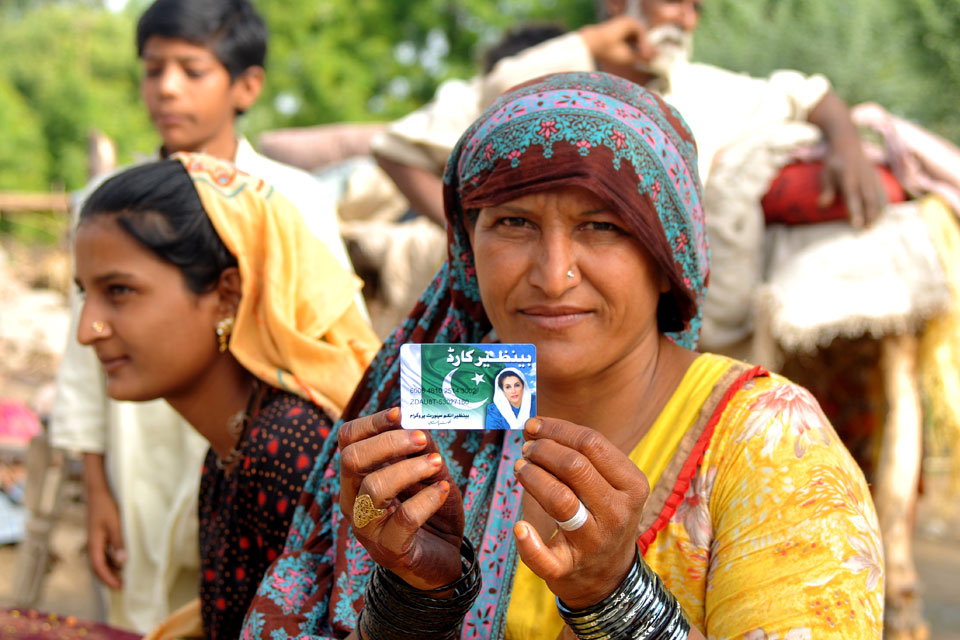
\includegraphics[width=7cm,height=5cm]{bisp-bdc}
		Pre-treatment: Debit card
		\end{column} 

		\begin{column}{0.5\textwidth}
		\center 
		{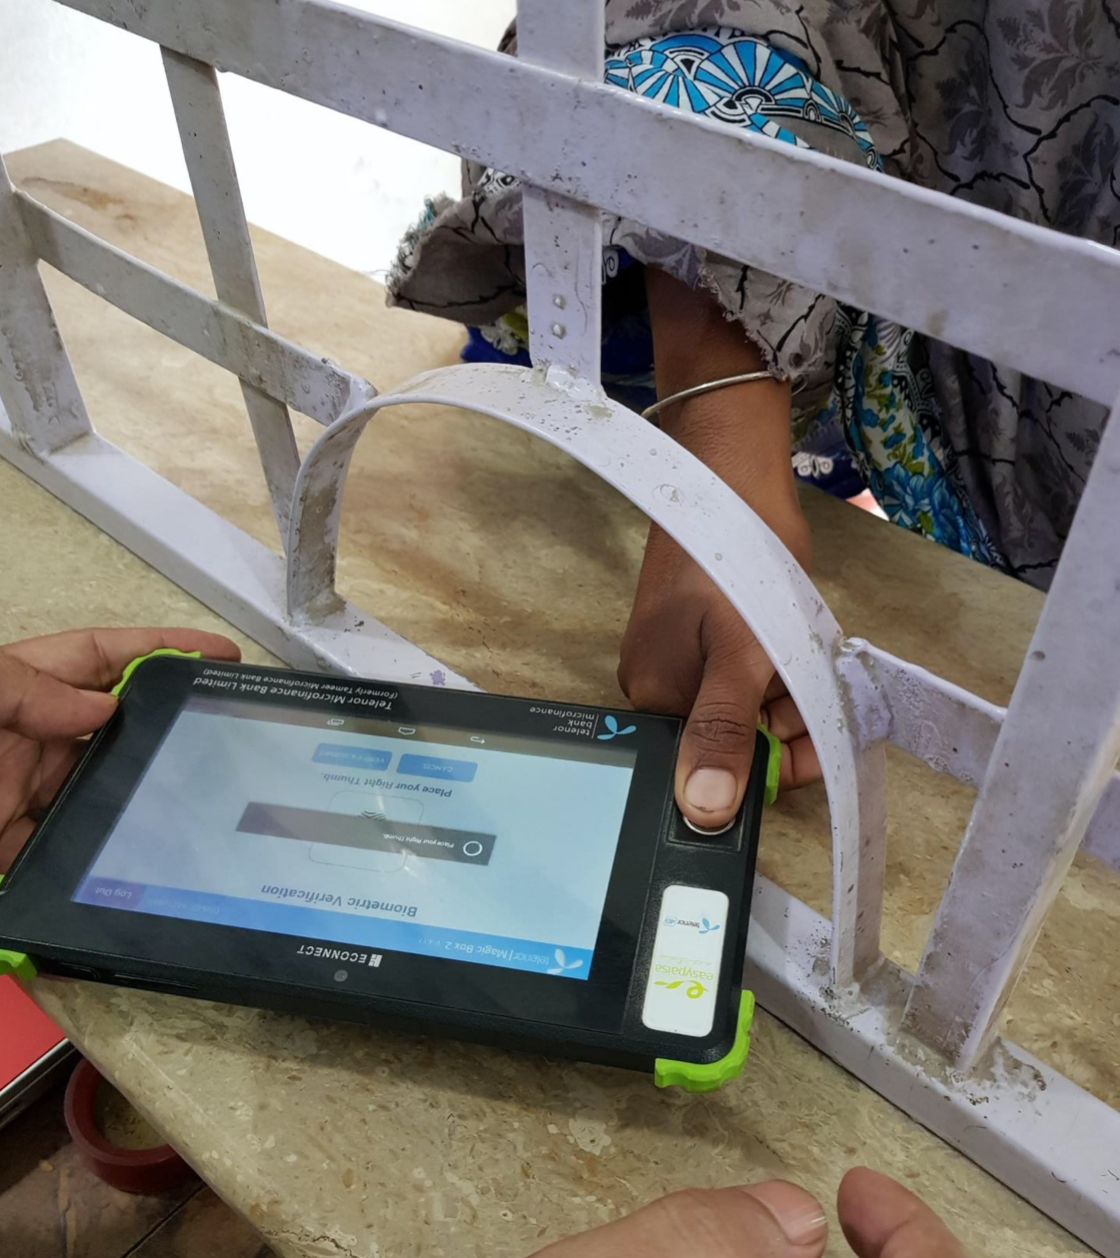
\includegraphics[width=7cm,height=5cm]{authentication}} \\
		Post-treatment: Biometric verification 
		\end{column} 

	\end{columns}
	\headlineextra{\footnotesize \textcolor{white}{Do not circulate}}
\end{frame} 


%------------------------------------------------------------------------

\begin{frame}{BVS reform had four main consequences for the payment system}
	\centering
	\textbf{2. Recipient present: Woman has to visit payment point to scan fingerprint}
	\begin{columns}
		\begin{column}{0.5\textwidth}
		  \begin{figure}
			  \begin{center}
				  {{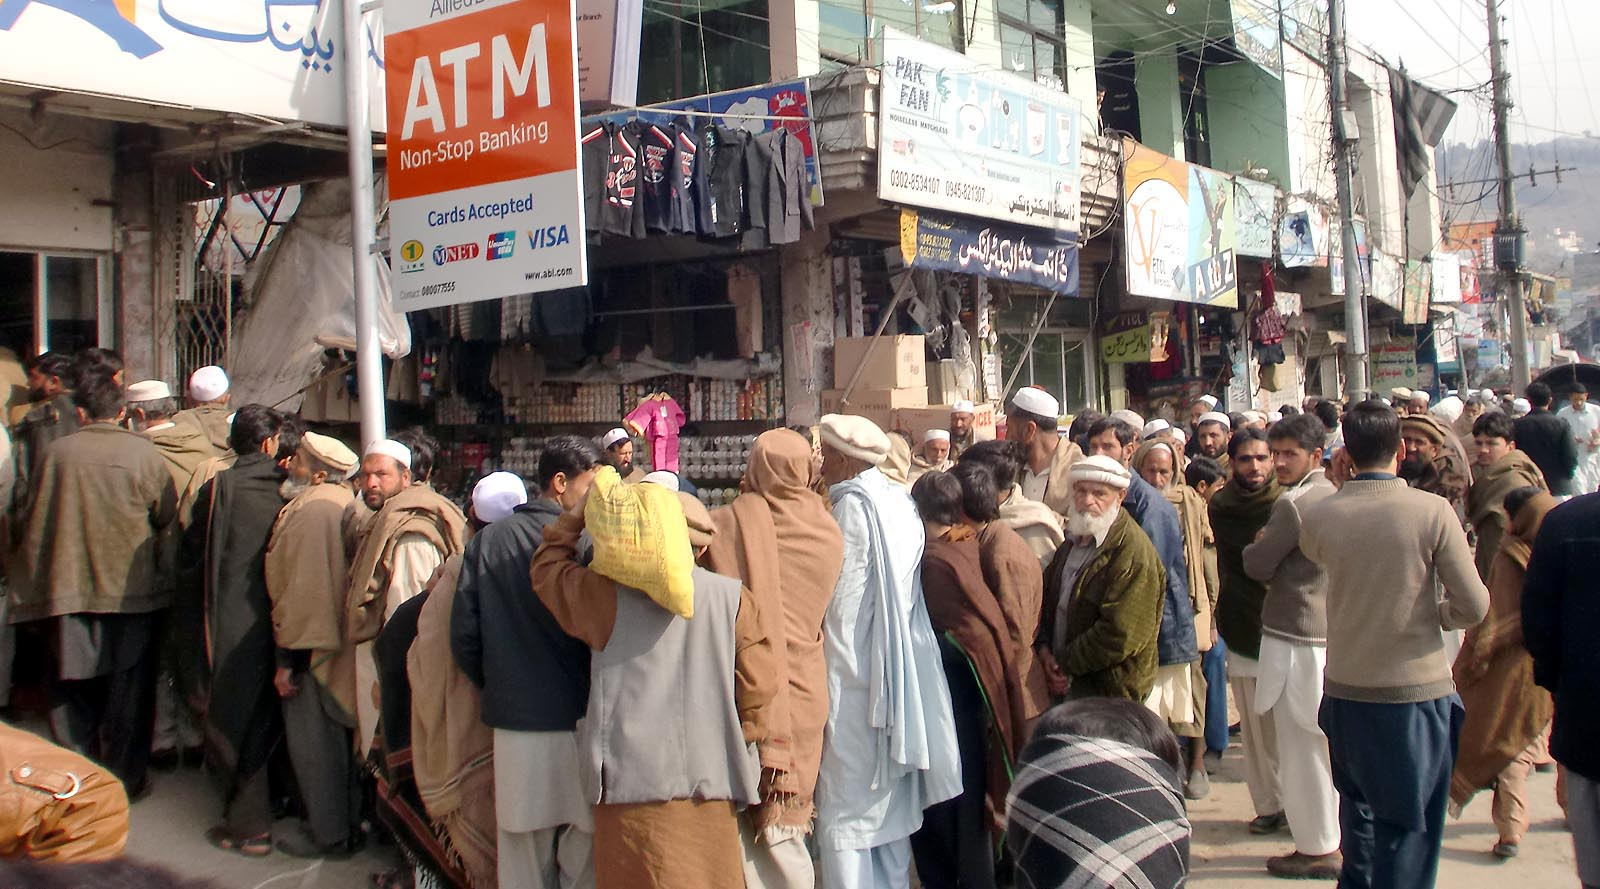
\includegraphics[width=7cm,height=5cm]{male-withdrawal}}} \\
				  Pre-treatment: Men in line to withdraw BISP cash 
			  \end{center}
			\end{figure} 
		\end{column} 

		\begin{column}{0.5\textwidth}
		\begin{figure} 
			  \begin{center}
				  {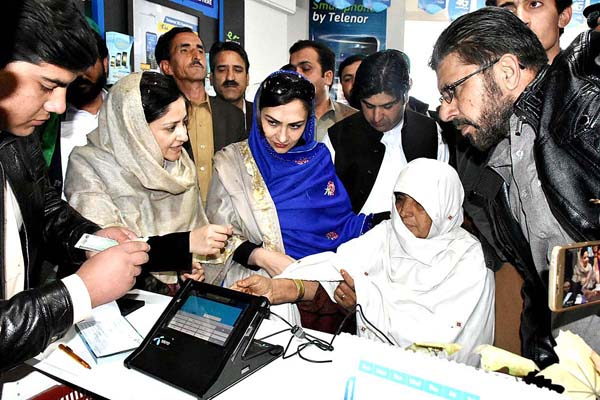
\includegraphics[width=7cm,height=5cm]{bisp-bvs}} \\
				  Post-treatment: women must be present to scan their fingerprints 
			  \end{center}
		  \end{figure}
		\end{column}
	\end{columns}

	\headlineextra{\footnotesize \textcolor{white}{Do not circulate}}
\end{frame} 


%------------------------------------------------------------------------

\begin{frame}{BVS reform had four main consequences for the payment system}
	\centering
	\textbf{3. Human involvement: Some areas move from machine (ATM) to human retail agent}
	
	\begin{columns}

		\begin{column}{0.5\textwidth}
		\center 
		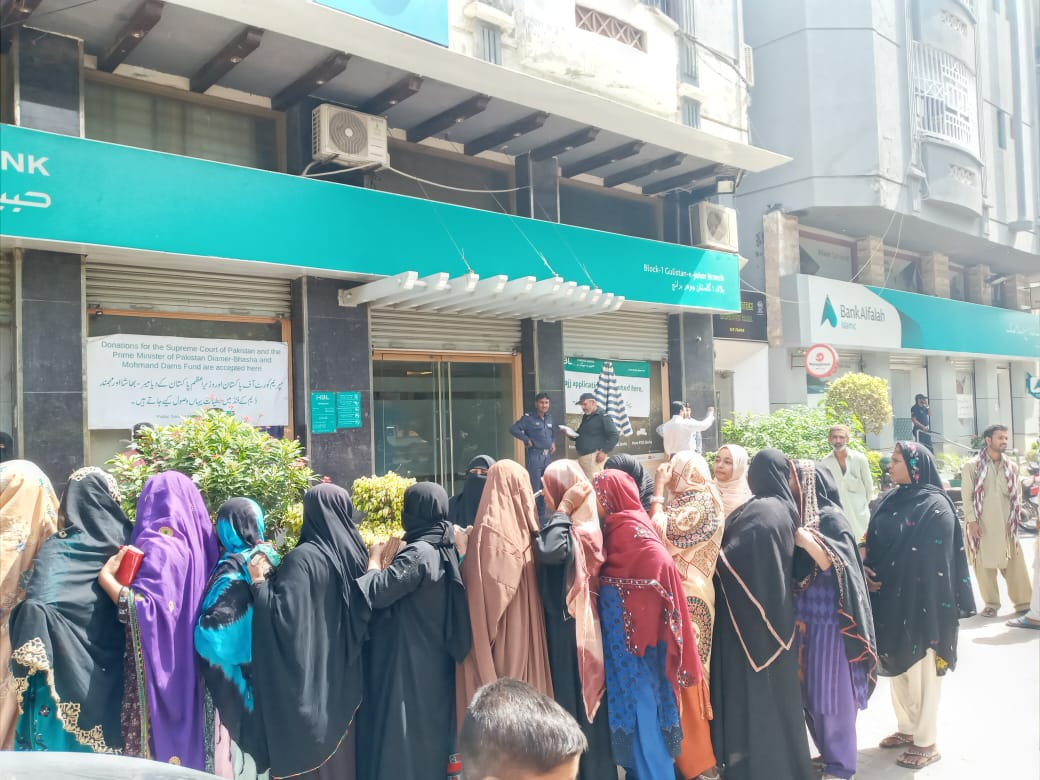
\includegraphics[width=7cm,height=5cm]{bisp-withdrawal-from-banks}
		ATMs 
		\end{column} 
		\begin{column}{0.5\textwidth}
		\center 
		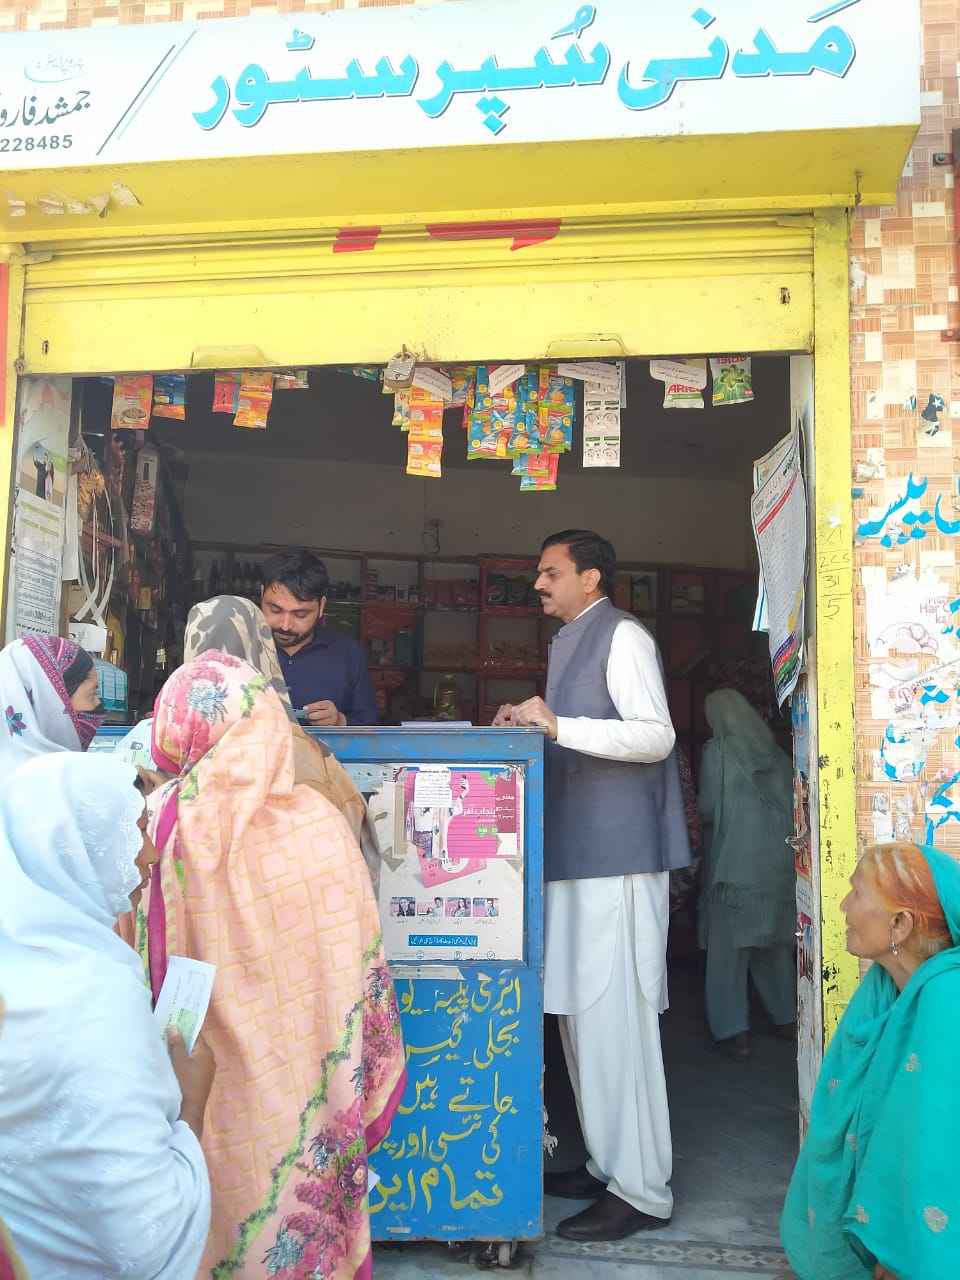
\includegraphics[width=6cm,height=5cm]{bisp-pos}

		``Point of sale" retail agents
		
		\end{column} 


	\end{columns}
	\headlineextra{\footnotesize \textcolor{white}{Do not circulate}}
\end{frame} 

\begin{frame}{BVS reform had four main consequences for the payment system}
	\centering
 	\textbf{4. Coverage: Possible increase in number of human retail agents}
	\begin{columns}

		\begin{column}{0.5\textwidth}
		\center 
		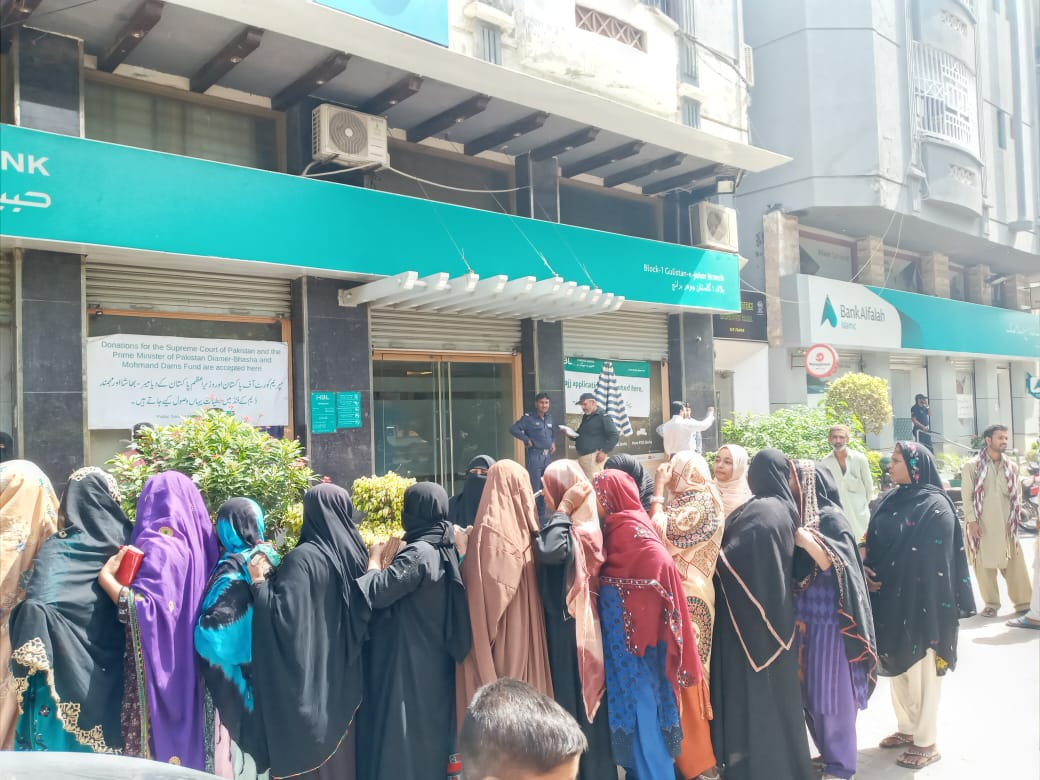
\includegraphics[width=7cm,height=5cm]{bisp-withdrawal-from-banks}
		ATMs 
		\end{column} 
		\begin{column}{0.5\textwidth}
		\center 
		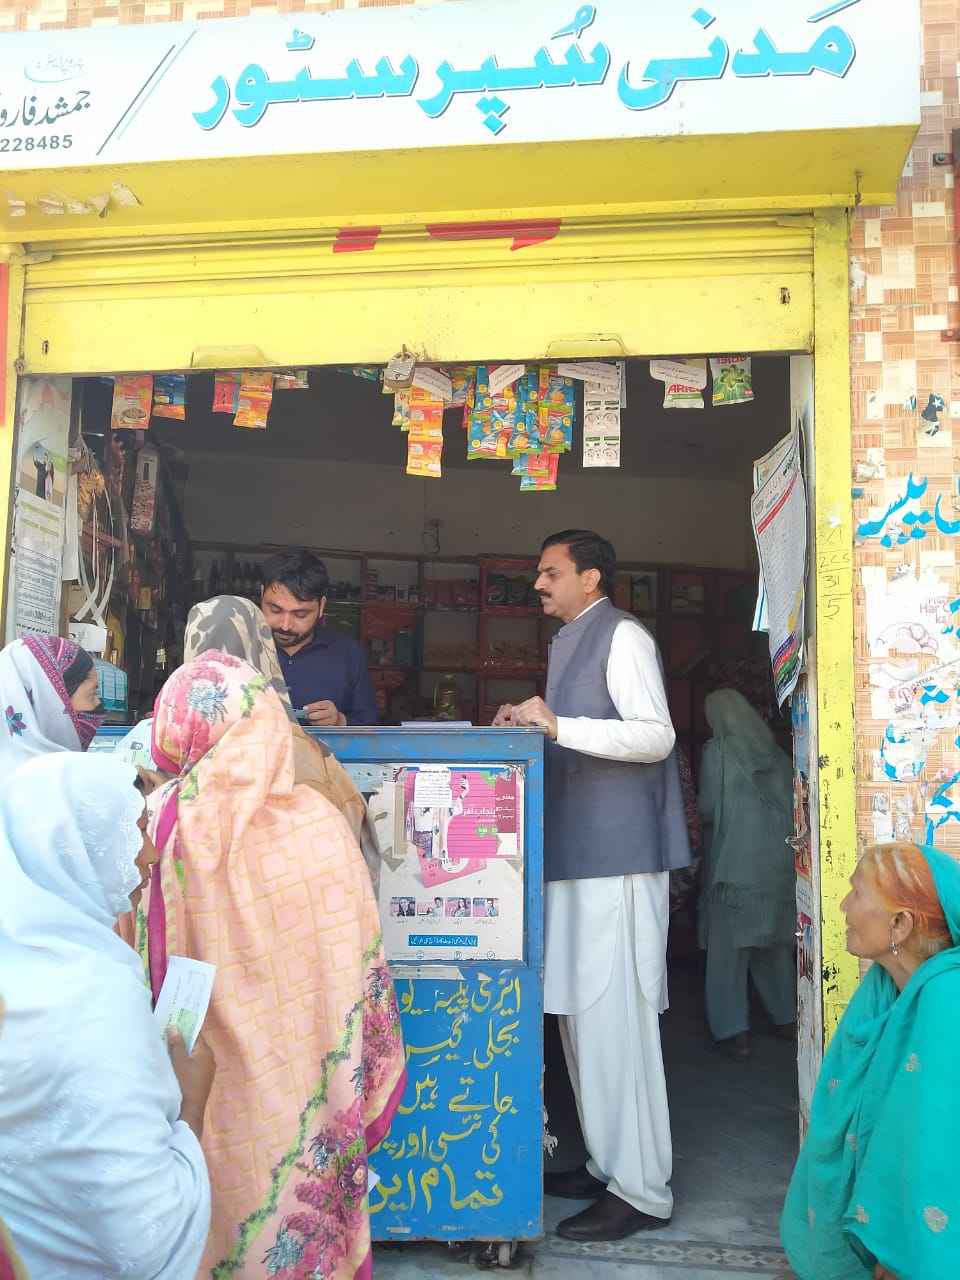
\includegraphics[width=6cm,height=5cm]{bisp-pos}

		``Point of sale" retail agents
		
		\end{column} 


	\end{columns}
	\headlineextra{\footnotesize \textcolor{white}{Do not circulate}}
\end{frame} 

%------------------------------------------------------------------------




%------------------------------------------------------------------------

\begin{frame}{Goals and preview of findings}
\headlineextra{\footnotesize \textcolor{white}{Do not circulate}}
Goals:
\begin{enumerate}
	\setlength\itemsep{1em}
	\item[A.] \textbf{Estimate total effect} of reform
	\item[B.] \textbf{Unpack mechanisms} behind the results 
\end{enumerate}
\pause\vspace{.3cm}

Preview of findings:
	\begin{itemize}
		\setlength\itemsep{2em}
		\item \textbf{Biometric technology} appears to have \textbf{no effect on net cash received} 
		\pause 
		\item Effect partly explained by increased side-payments to human retail agents 
		\pause 
		\item For \textbf{mobility constrained women}, biometric 		verification systems \textbf{increased control over cash} 
	\end{itemize}
\end{frame} 

%%%%%%%%%%%%%%%%%%%%%%%%%%%%%%%%%%%%%%%%%%%%%%%%%%%%%%%%%%%%%%%%%%%%%%%%%

\section{Empirical strategy and data}
\frame{\tableofcontents[currentsection]}

\begin{frame}{Staggered rollout of BVS reform}
\small Each district switched to BVS as local administration and banks were ready 
to do so 
	\centering
	\vspace{-.1cm}
			{\scalebox{.86}{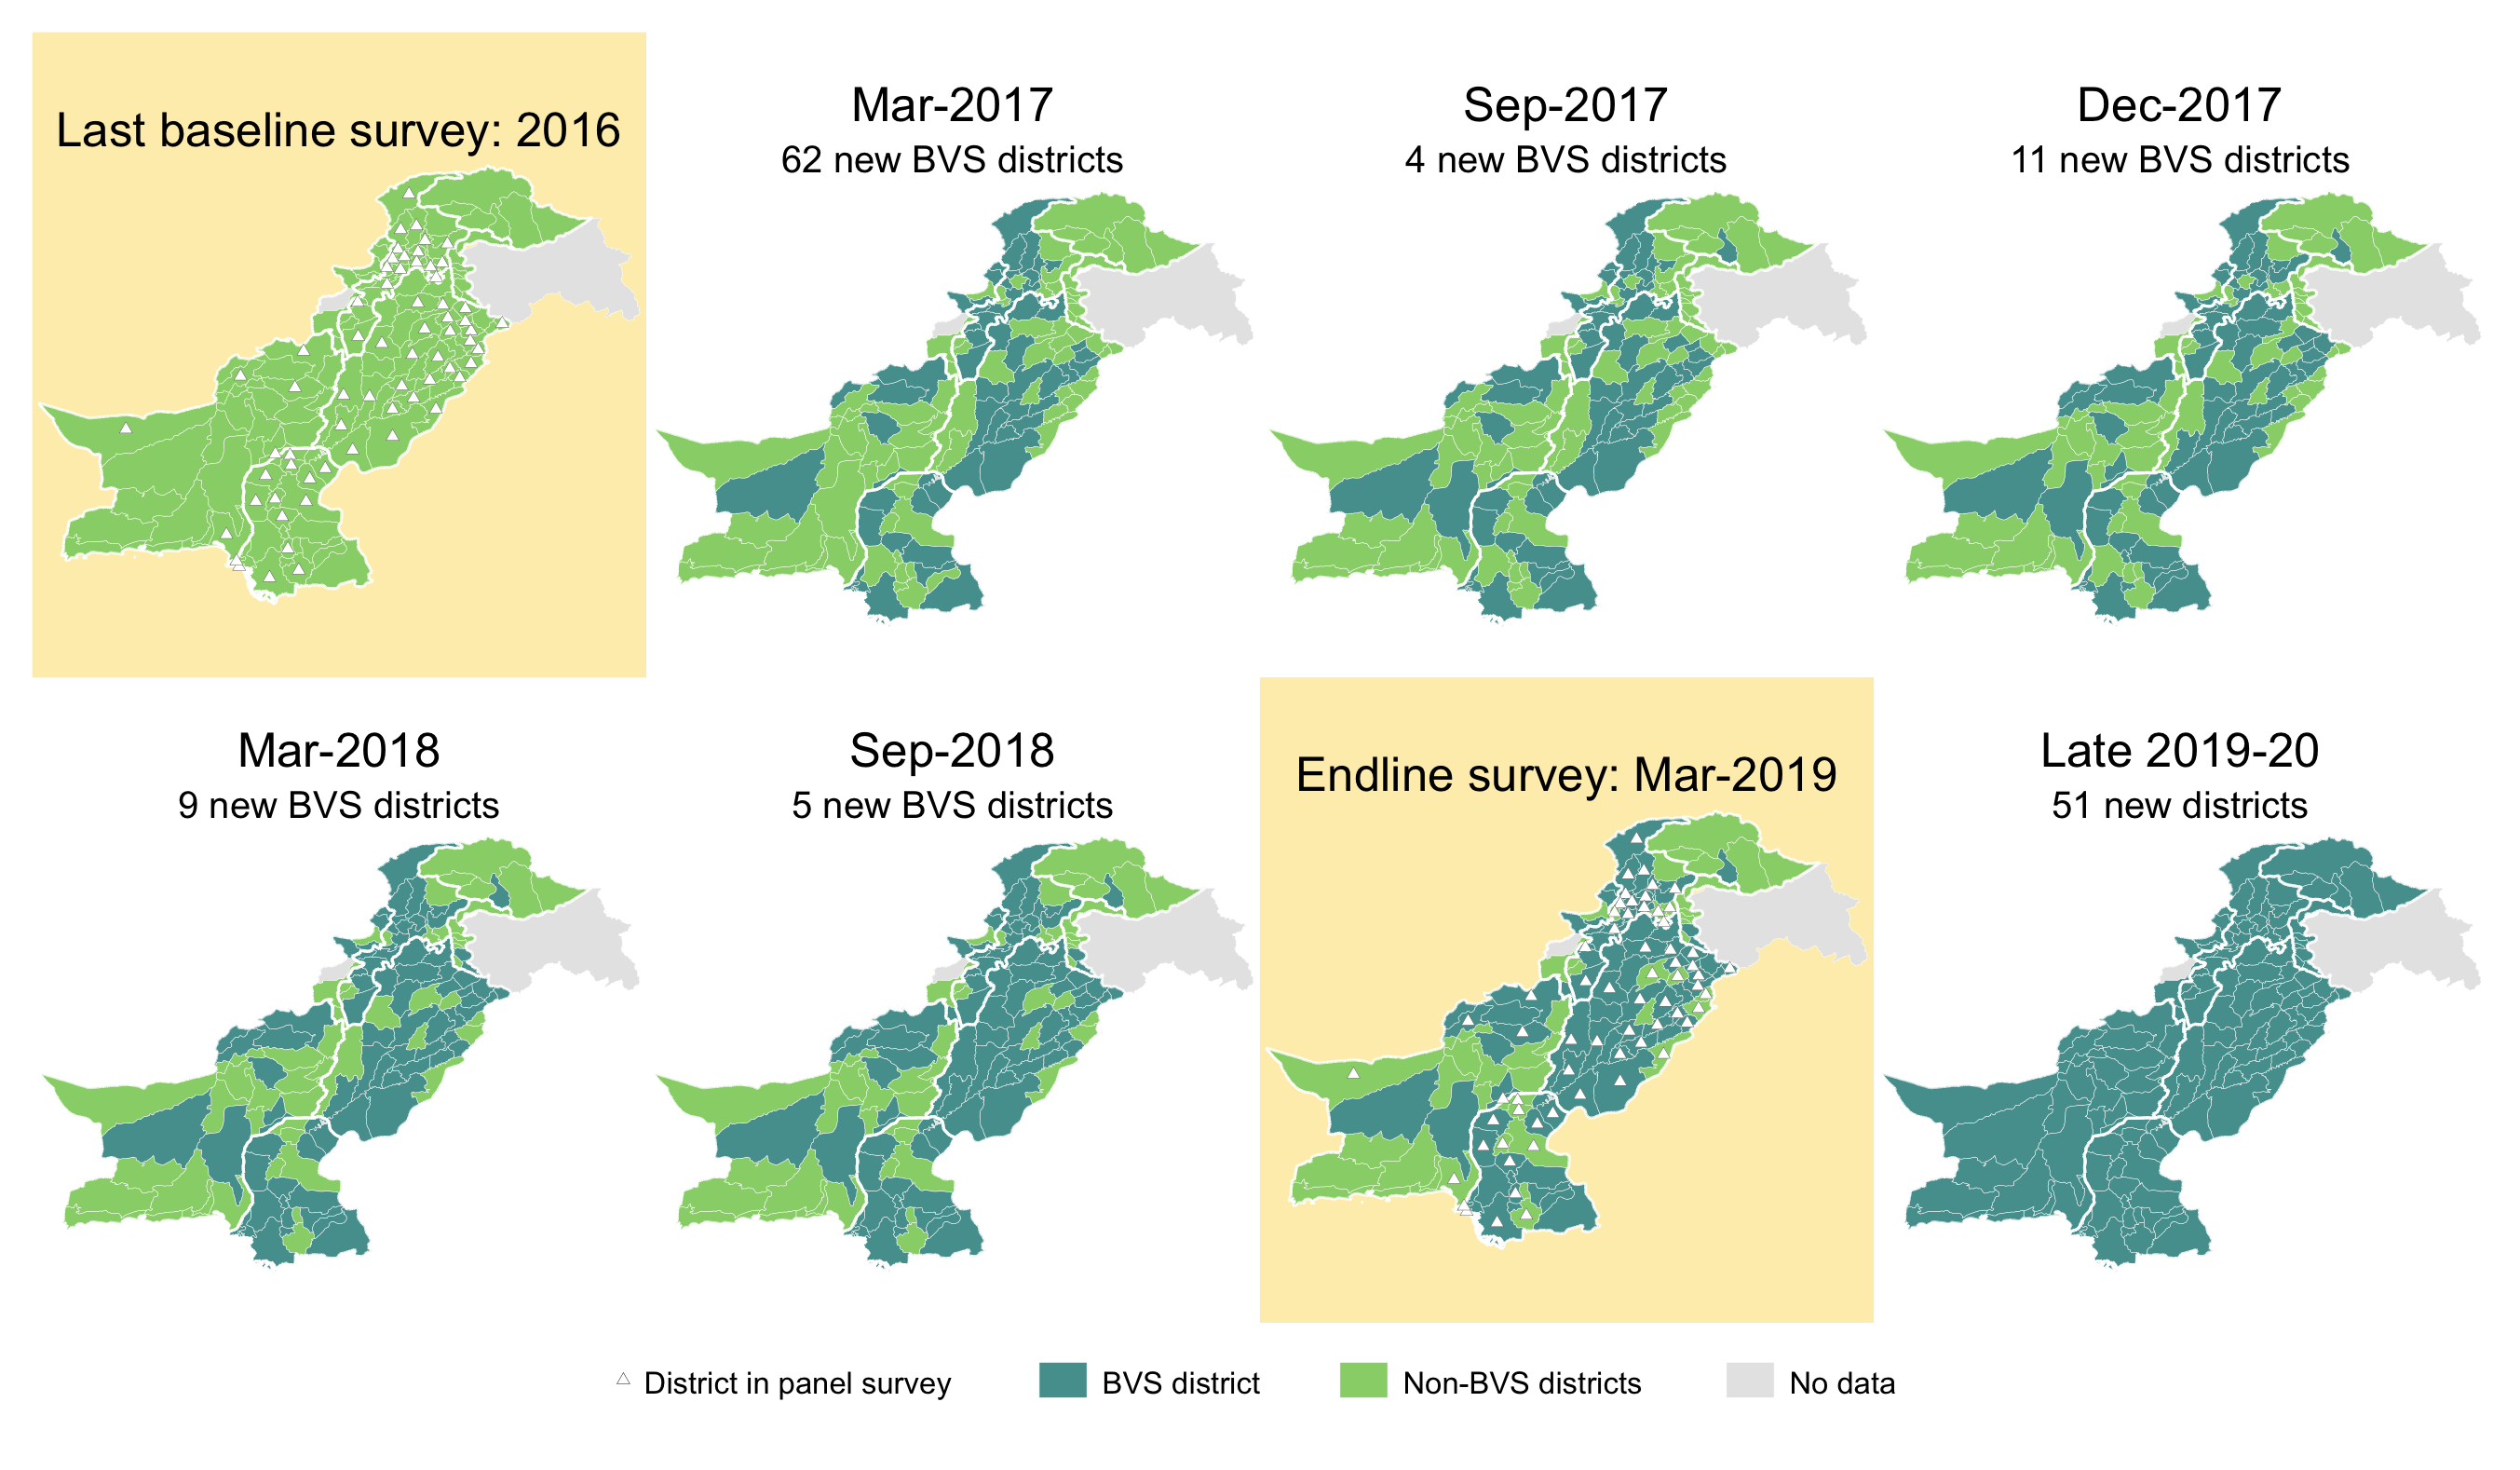
\includegraphics{BVS_transition_series}}} 
	\headlineextra{\footnotesize \textcolor{white}{Do not circulate}}
\end{frame}

\begin{frame}[label=methodology]{Methodology}
	\headlineextra{\footnotesize \textcolor{white}{Do not circulate}}
	\begin{itemize}
			\setlength\itemsep{1.5em}
			\item We study the staggered \textbf{roll-out of the 
			biometric verification system (BVS)} across Pakistan
			\pause
			\item Difference-in-differences: Compare outcomes 
			\textbf{before and after BVS} of households that are in 
			\textbf{BVS early vs. late implementation areas} 
			\item \textbf{Identifying assumption:} in the absence of treatment 
			the outcomes would have evolved similarly in the early and late 
			implementation districts
			\item Under this assumption, estimated effects are \textbf{causal
			 effect of BVS transition} 
			 \pause
			 \item Areas with early, middle and late 
 			BVS transition were \textbf{similar at baseline}  
 			\hyperlink{balance}{\beamergotobutton{Table}} and had \textbf{similar 
 			time trends} over \textbf{several pre-treatment rounds} 
	\end{itemize}
\end{frame}


%-------------------------------------------------------------------------

\begin{frame}[label=survey]{Data}
\textbf{\underline{Data source 1}}\\
\vspace{.6cm}
Panel survey collected by OPM for evaluation of BISP cash transfer: 
\begin{itemize} 
		\setlength\itemsep{1.5em}
		\item Four rounds, 2013-2019 
		\item Nation-wide (63 districts)
		\item One beneficiary woman interviewed per HH 
		\item \textbf{No differential 
		attrition} by treatment \hyperlink{attrition}{\beamergotobutton{Table}}
		\item Analysis sample: \textbf{balanced panel of beneficiaries}, about 
		\textbf{2,800 BISP beneficiary HHs}
\end{itemize} 
\headlineextra{\footnotesize \textcolor{white}{Do not circulate}}
\end{frame} 

%-------------------------------------------------------------------------


\begin{frame}{Data}
\textbf{\underline{Data source 2}}\\
\vspace{.6cm}
\textbf{Administrative data} on payments and payment points (work in progress) 
		\vspace{.5cm}

\begin{itemize} 
		\setlength\itemsep{2em}
	\item 9000+ BISP beneficiaries that ever appeared in the OPM sample
	\item Data on all deposits and withdrawals between 2015 and 2019 
	\vspace{.2cm}
		\begin{itemize}
			\item To be used to test for \textbf{discrepancies} in admin 
			  data versus self report 
		\end{itemize}
	\item Data on payment point locations used for each withdrawal by each 
	beneficiary
	\vspace{.2cm}
	\begin{itemize}
		\item To be used to test for \textbf{market power / competition} 
		effects
	\end{itemize}
\end{itemize}
\headlineextra{\footnotesize \textcolor{white}{Do not circulate}}
\end{frame} 

%-------------------------------------------------------------------------

\begin{frame}{Estimation}
	\begin{equation*}
		Y_{idt} = \alpha + \beta BVS_{dt} + \lambda_{i} + \tau_{pt} +\epsilon_{idt}
	\end{equation*}
	 
	\begin{itemize}
		\item $Y$ is any outcome of interest for household $i$ in district 
		$d$ and survey round $t$ 
		\item $BVS_{dt}$ treatment indicator (BVS in use) 
		\item $\lambda_{i}$ household fixed effects 
		\item $\tau_{pt}$ province-year fixed effects 
		\item Standard errors clustered by district (level of rollout) 
	\end{itemize} 
		\vspace{.5cm}


		\headlineextra{\footnotesize \textcolor{white}{Do not circulate}}
\end{frame} 

\begin{frame}{Outcomes}

We registered a PAP for analysis \textbf{before PIs had access to endline data} (EGAP 20200212AB) 
		
\begin{enumerate}
        \item \textbf{*Cash disbursement:} \% of transfer withdrawn; delays between withdrawals (admin \& survey data)
\pause
\vspace{.2cm}
        \item \textbf{*Cash received by recipient HHs:} \% of cash transfer received; amt. of side payment (survey data) 
\pause
\vspace{.2cm}

        \item \textbf{**Recipient present:} whether woman is present at payment point
\pause
\vspace{.2cm}

        \item \textbf{*Costs of withdrawal:} time \& money spent on collecting most recent transfer (survey data)
\pause
\vspace{.2cm}
        
        \item \textbf{*Female control over cash:} recipient decides how transfer is spent; involved in decisons over household spending \& own earnings; spending on clothing, education, healthcare, male temptation goods (survey data)    
\pause
\vspace{.2cm}

        \item \textbf{Satisfaction:} whether recipient is satisfied with the payment method
\pause
\vspace{.2cm}

        \item \textbf{*Female mobility:} recipient able to travel to market, doctor, friends, family, place of worship (survey data)
\pause
\vspace{.2cm}

        \item \textbf{*Female empowerment:} decisions over healthcare; voting; labor force participation
        
\end{enumerate}
\end{frame}

%%%%%%%%%%%%%%%%%%%%%%%%%%%%%%%%%%%%%%%%%%%%%%%%%%%%%%%%%%%%%%%%%%%%%%%%%


\section{Results}


\begin{frame}{1. Rollout of BVS strongly predicts BVS transactions}
	\centering
	\begin{table}
		\caption{\textbf{Use of BVS for withdrawals (at endline)}}
		\scalebox{.95}{\input{\tabdir 8_firststage_predict_treatment_v2.tex}}
	\end{table}
	\headlineextra{\footnotesize \textcolor{white}{Do not circulate}}
\end{frame} 

%-------------------------------------------------------------------------

\begin{frame}{Rollout of BVS shifts people from ATM to human retail agent}
\begin{figure}
	\vspace{-.39cm}
	\caption{Made a withdrawal in tranche \emph{t} using human retail agent}
	\begin{center}
	  \vspace{-.157cm}
	  {\scalebox{.74}{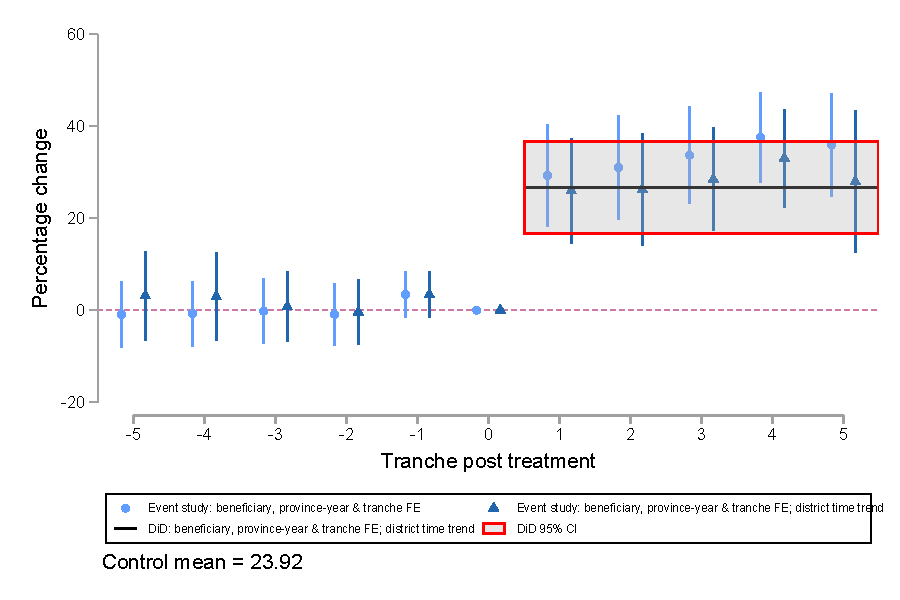
\includegraphics{coefplots/MIS_POS_recenter}}} \\
	\end{center}
\end{figure}
\end{frame} 

%-------------------------------------------------------------------------

\begin{frame}{2. Recipient more likely to be present at payment point}
	\headlineextra{\footnotesize \textcolor{white}{Do not circulate}}
	\vspace{-.4cm}
	\begin{columns}
		\begin{column}{0.55\textwidth}
		  \begin{figure}
			  \begin{center}
				  \vspace{-.25cm}
				  {\scalebox{.68}{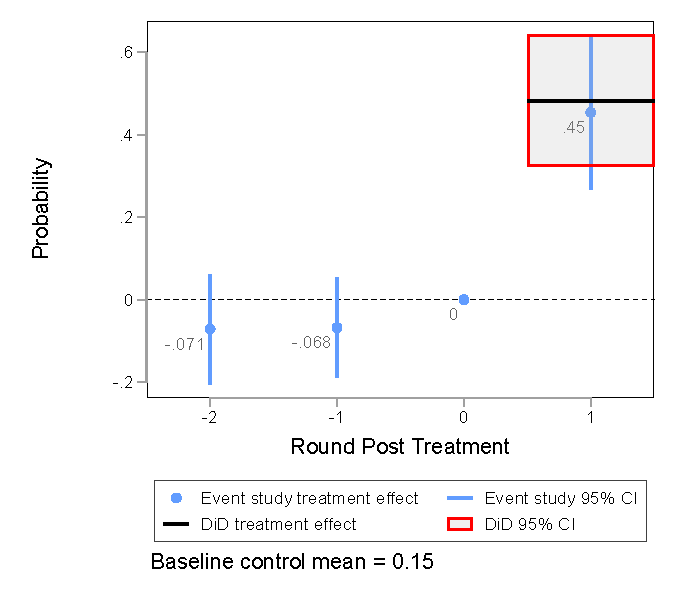
\includegraphics{coefplots/ES_DD_JQ04A_0}}} \\
			  \end{center}
			  \vspace{-.2cm}
			  {\tiny Note: The graph shows regression coefficients, 
			  controlling for household and province-year fixed 
			  effects. Standard errors clustered at the 
			  district level. \par}
		  \end{figure}
		\end{column}
		\begin{column}{0.45\textwidth}
		\begin{itemize}
			\setlength\itemsep{2em}
			\item Pre-treatment, \textbf{49\%} of women reported they are 
			\textbf{not allowed to go alone} to any of: market, clinic, 
			friend's home, nearby shrine / mosque
			\pause
			\item In the baseline control group, only \textbf{15\% of women 
			are present at payment points when their cash is collected}
			\pause
			\item BVS  \textcolor{green}{\textbf{increases}} women's 
			probability of \textbf{attending cash withdrawal in person} by 
			\textcolor{green}{\textbf{46.2}} percentage points
			\pause
			\item They may 
			still be accompanied (not observed in data) 
		 \end{itemize}
		\end{column}
	\end{columns}
\end{frame}






\begin{frame}[label=sidepayments]{3. Cash received} 
	\begin{center}
		\vspace{-.25cm}
		{\scalebox{.74}{%
		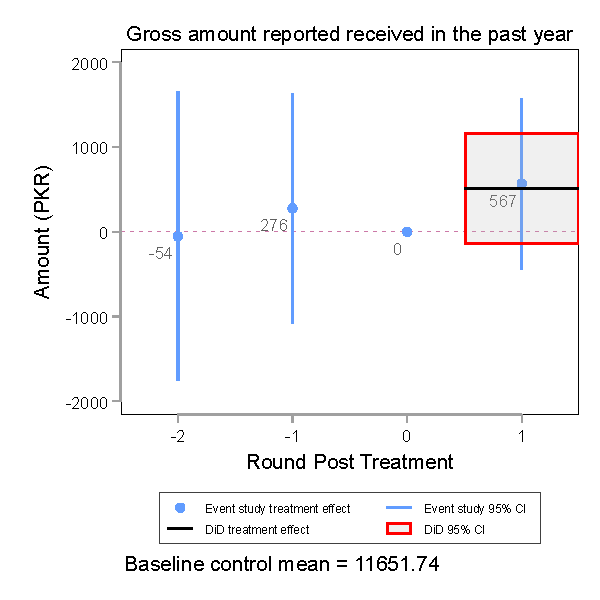
\includegraphics{coefplots/ES_DD_wins_JQ03}}} 
		\hyperlink{map}{\beamergotobutton{Map: increase in side payments}}
		\hyperlink{bargraph}{\beamergotobutton{Bar graph: magnitude}} 
	\end{center}					
	\headlineextra{\footnotesize \textcolor{white}{Do not circulate}}
\end{frame}

\begin{frame}[label=sidepayments]{4. Travel cost and side payments}
	\centering
	\begin{columns}

		\begin{column}{0.5\textwidth}
		\center 
		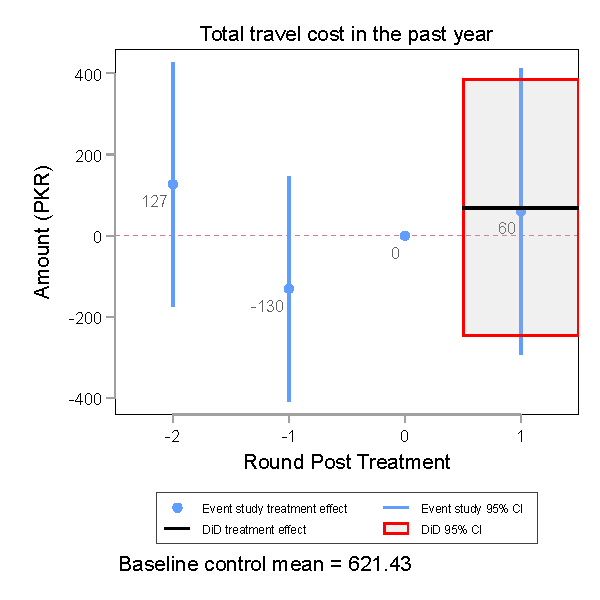
\includegraphics[width=7cm,height=7cm]{coefplots/ES_DD_total_travel_cost}
		\end{column} 

		\begin{column}{0.5\textwidth}
		\center 
		{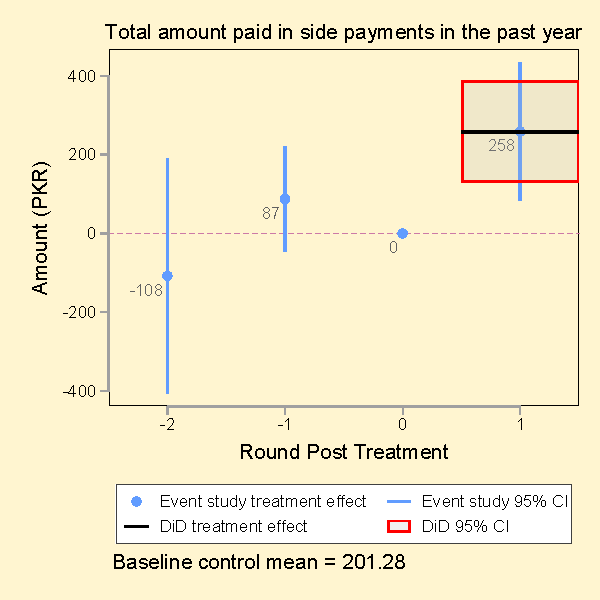
\includegraphics[width=7cm,height=7cm]{coefplots/ES_DD_total_bribes}} \\
		\end{column} 

	\end{columns}
	\headlineextra{\footnotesize \textcolor{white}{Do not circulate}}
\end{frame} 


\begin{frame}[label=desc_graph]{Most side payments paid to retail agents}
	\begin{center}
		\scalebox{.62}{\hspace{-.1cm}%
		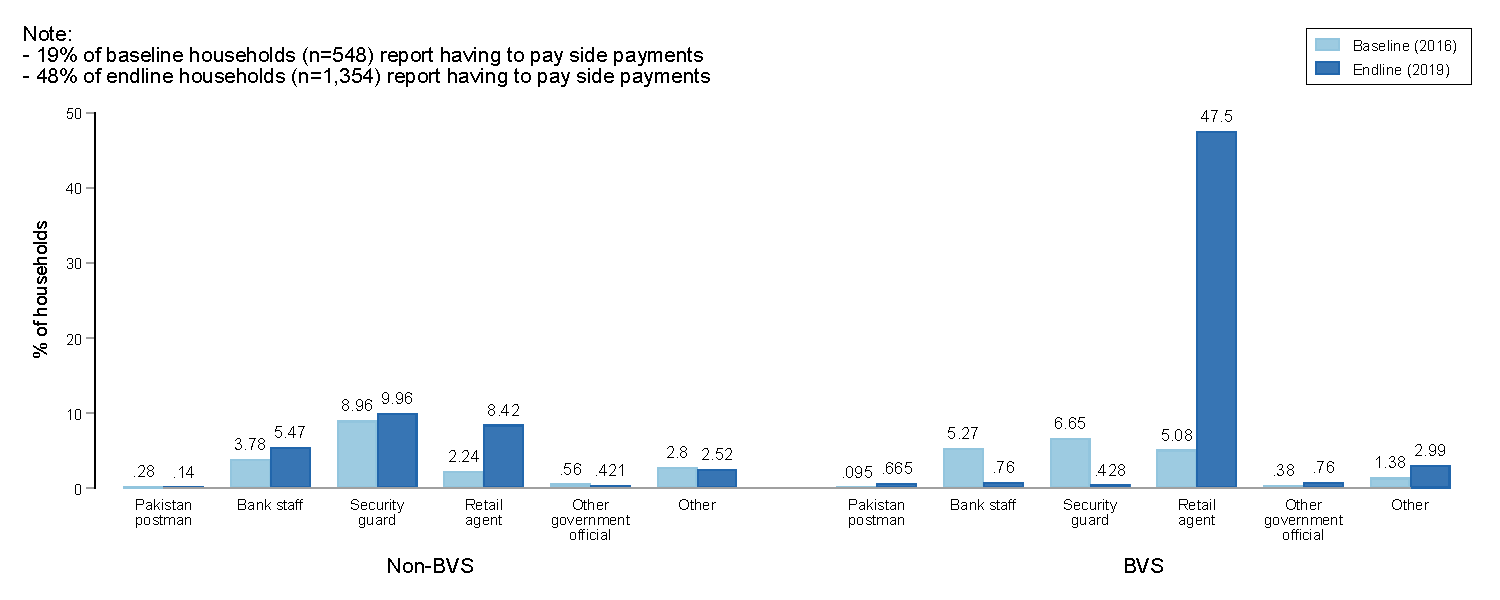
\includegraphics{panel_JQ12_side_payments_paid_to.pdf}} 
	\end{center}
	\hyperlink{pos_hte}{\beamergotobutton{Back}}
	\headlineextra{\footnotesize \textcolor{white}{Do not circulate}}
\end{frame}


\begin{frame}[label=sidepayments]{Net cash received} 
	\begin{center}
		\vspace{-.25cm}
		{\scalebox{.74}{%
		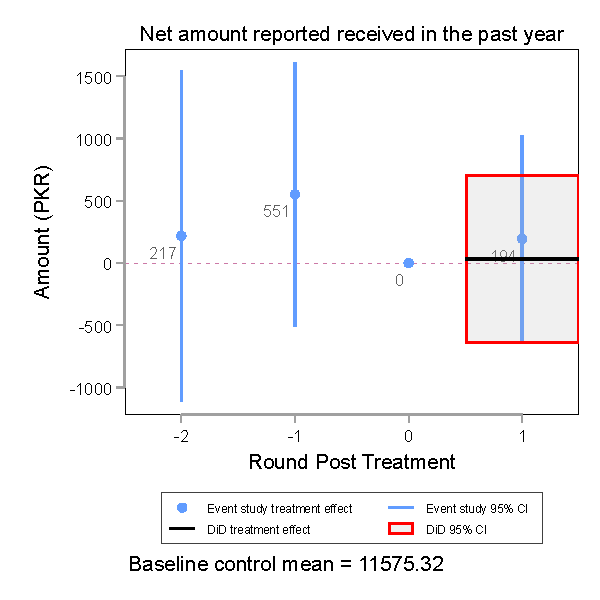
\includegraphics{coefplots/ES_DD_net_amt_rcvd}}%
		\vspace{-.2cm}} 
		\hyperlink{map}{\beamergotobutton{Map: increase in side payments}}
		\hyperlink{bargraph}{\beamergotobutton{Bar graph: magnitude}} 
	\end{center}					
	\headlineextra{\footnotesize \textcolor{white}{Do not circulate}}
\end{frame}




\begin{frame}[label=control_map]{5. Control over cash: large increases}
	\headlineextra{\footnotesize \textcolor{white}{Do not circulate}}
	\begin{columns}
		
		\begin{column}{0.5\textwidth}
			\small
			\textbf{All women}:
			Weak evidence that BVS \textcolor{green}{\textbf{increases 
			reported control}} of transfer by \textbf{7.5} percentage points 
			\footnotesize[ \emph{p}-value: .022 ]
			\hyperlink{control}{\beamergotobutton{Map}}
			\vspace{-.2cm}
		  \begin{center}
			  {\scalebox{.6}{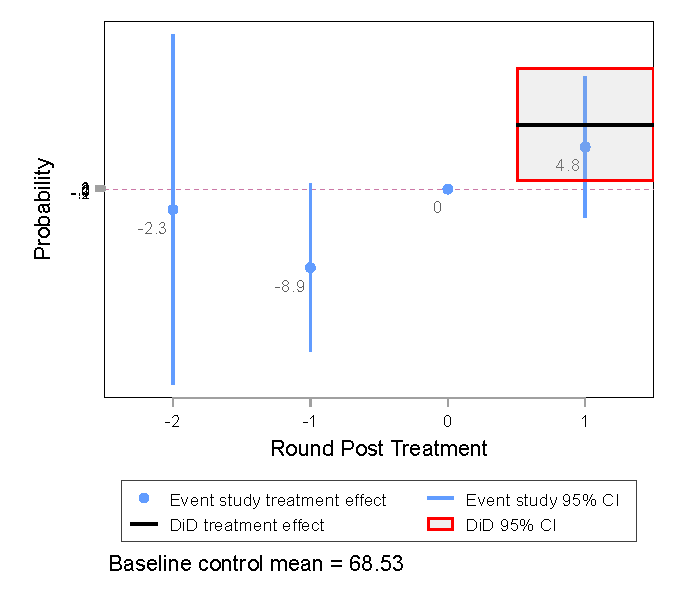
\includegraphics{coefplots/ES_DD_JQ18A_1}}} \\
		  \end{center}
		\end{column}
		\pause
		\begin{column}{0.5\textwidth}
			\small
			\textbf{Women who did not pick up cash at baseline}: Strong evidence
			in subsample that BVS \textcolor{green}{\textbf{increases reported 
			control}} of transfer by \textbf{10} percentage points 
			\footnotesize[ \emph{p}-value: 0.015 ]
			\vspace{-.2cm}
			\begin{center}
			  {\scalebox{.6}{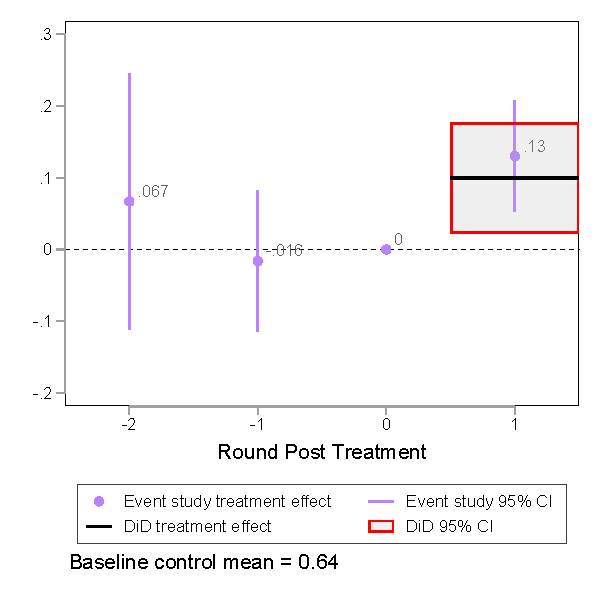
\includegraphics{coefplots/ES_DD_HT_JQ18A_1}}} \\
		  \end{center}
		\end{column}
	\end{columns}
			  {\tiny Note: The graph shows regression coefficients, 
			  controlling for household and province-year fixed effects.
			  Standard errors are robust and clustered at the 
			  district level. \par}
\end{frame}



%-------------------------------------------------------------------------
\begin{frame}[label=satisfaction]{6. Satisfaction: large  decrease in satisfaction with payment system}
	\begin{columns}
		\begin{column}{0.6\textwidth}
		  \centering
		  \vspace{-.157cm}
		  {\scalebox{.7}{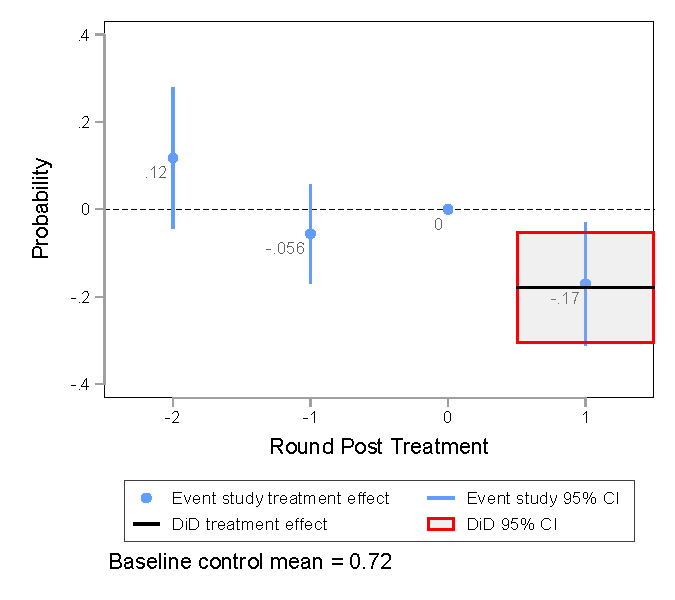
\includegraphics{coefplots/ES_DD_JQ15_1}}} \\
		  {\tiny Note: The graph shows regression coefficients, 
		  controlling for household and province-year fixed effects.
		  Standard errors clustered at the 
		  district level. \par}
		\end{column}
		\hspace{-.9cm}
		\begin{column}{0.4\textwidth}
			BVS transition \textbf{decreased proportion of women who
			report they are ``very satisfied"} with the payment method by
			\textcolor{maroon}{\textbf{17.9}} percentage points  
			\end{column}
	\end{columns}
	\headlineextra{\footnotesize \textcolor{white}{Do not circulate}}
\end{frame}



 \begin{frame}[label=decay]{Unintended consequences of BVS did not disappear after 
	 several payment tranches}
	 \begin{columns}
	 \begin{column}{0.5\textwidth}
	   \begin{center}
		   Total side payments paid 
		   {\scalebox{.6}{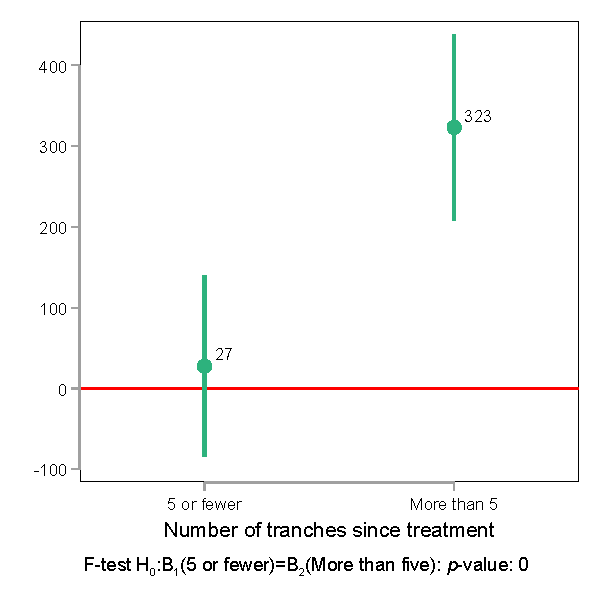
\includegraphics{coefplots/decay_total_bribes}}} \\
	   \end{center}
	 \end{column}
	 \begin{column}{0.5\textwidth}
		 \begin{center}
		   Very satisfied with payment method
		   {\scalebox{.6}{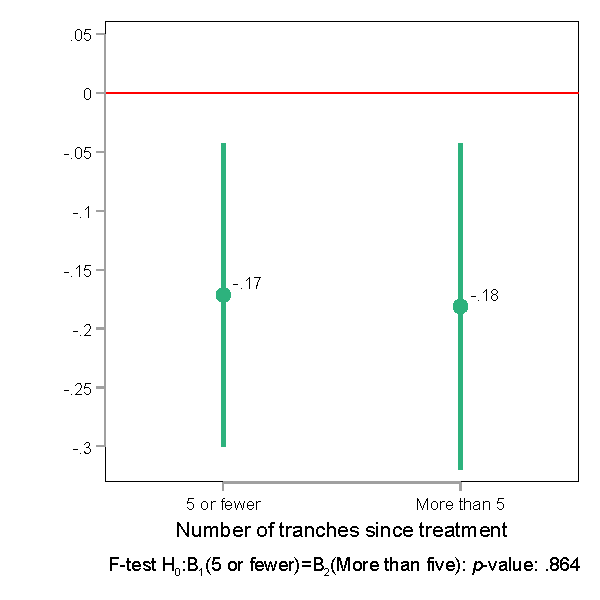
\includegraphics{coefplots/decay_JQ15_1}}} \\
	   \end{center}
	 \end{column}
 \end{columns}
		   {\tiny Note: The graph shows regression coefficients, 
		   controlling for household and province-year fixed effects.
		   Standard errors clustered at the 
		   district level. \par}
 \headlineextra{\footnotesize \textcolor{white}{Do not circulate}}
 \hyperlink{balance}{\beamergotobutton{Balance by treatment rollout}}

 \end{frame} 


\section{Unpacking mechanisms}
\frame{\tableofcontents[currentsection]}
\begin{frame}{Unpacking mechanisms: delivery of cash}
\headlineextra{\footnotesize \textcolor{white}{Do not circulate}}
Impacts of the BISP biometrics reform could be driven by four main mechanisms: 
\vspace{.3cm}
\begin{enumerate}
	\setlength\itemsep{1em}
	\item[1.] \textbf{ID requirement:} Biometric authentication instead of debit card
\pause
	\item[2.] \textbf{Recipient present:} Woman has to visit payment point to scan fingerprint
\pause
	\item[3.] \textbf{Human involvement:} Some areas move from machine (ATM) to human retail agents
\pause
	\item[4.] \textbf{Coverage:} Possible increase in number of human retail agents
\end{enumerate} 
\end{frame}


%-------------------------------------------------------------------------

\begin{frame}{Biometric authentication instead of debit card}
\headlineextra{\footnotesize \textcolor{white}{Do not circulate}}
\vspace{-.4cm}
\begin{itemize}
\item Biometrics may reduce \textbf{account ``freezing''} due to card loss or wrong PINs 
\pause
\item Biometrics may prevent \textbf{card theft}
\pause
\item But biometrics may also exclude women with \textbf{depleted fingerprints or low mobility}
\pause 
\item All of these should be detectable on the \textbf{extensive} margin, i.e., 
inability to withdraw the entire tranche
\end{itemize}
\pause
\begin{figure}
	\caption{PKR 0 withdrawn in a given tranche}
	\begin{center}
		\scalebox{.5}{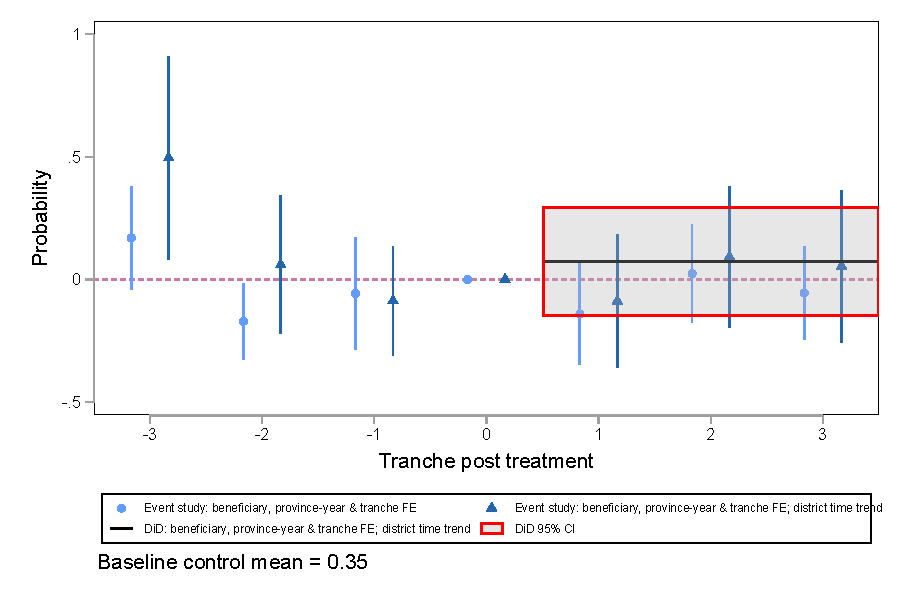
\includegraphics{coefplots/MIS+OPM_opm_zero_withdrawal_recenter}} 
	\end{center}
\end{figure}

\end{frame} 

%-------------------------------------------------------------------------

%\begin{frame}{Component [2/4]: Shifts many areas from ATM to human retail agents}
%\textcolor{red}{When we have it ready we should show the HTE for extensive margin 
%payment by POS at baseline or ATM at baseline}
%\begin{figure}
%	\caption{PKR 0 withdrawn in a given tranche in PSUs with baseline retail agent 
%   availability}
%	\begin{center}
%		\scalebox{.5}{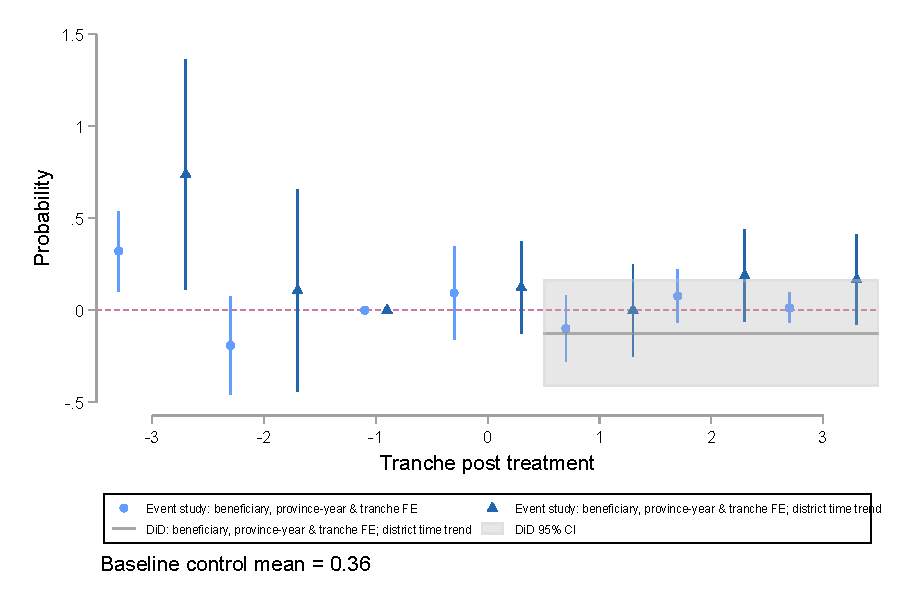
\includegraphics{coefplots/MIS+OPM_ht_pos_opm_zero_withdrawal}} 
%	\end{center}
%\end{figure}
%\end{frame} 

%-------------------------------------------------------------------------

\begin{frame}{Separating the effect of biometric authentication from effect of 
	machine-human switch}
	
\begin{table}[Changes in payment system varied]
\begin{tabular}{ccccc}
 & \multicolumn{2}{c}{Before} & After  \\
 & \textbf{POS + debit card} & \textbf{ATM + debit card} & \textbf{POS + BVS} \\
Transferable & Y & Y & N  \\
Human interaction & Y & N & Y
\end{tabular}
\end{table}
\pause

We compare treatment effects for two groups:
		\begin{itemize}
			\item Those who had access to human agent at baseline: addition of 
			biometrics 
			\item Those who had access to ATM at baseline:  addition of biometrics switch from ATM to human plus switch from ATM to human 
		\end{itemize} 
\end{frame}

\begin{frame}[label=gross]{Separating the effect of biometric authentication from effect of 
	machine-human switch}
	\begin{itemize}
		\item Large, robust \textcolor{green}{\textbf{increase}} in gross amount 
		for those \textbf{with baseline access to human retail agents}: adding 
		biometric authentication to human agents \textbf{increases amount received} 
		\item Effects similar (but noisier) for \textbf{net amount} 
		\hyperlink{net}{\beamergotobutton{Table}}	
	\end{itemize}

		\begin{table}
			\caption{\textbf{HTE by baseline access to human retail agents}}
			\scalebox{.6}{\input{\tabdir HT_POS_avail_gross_amount.tex}}
		\end{table}
	\headlineextra{\footnotesize \textcolor{white}{Do not circulate}}
\end{frame}


%-------------------------------------------------------------------------




\begin{frame}[label=pos_hte]{Separating the effect of biometric authentication 
	from effect of machine-human switch}
	\vspace{.2cm}
		\textcolor{red}{\textbf{Larger increase}} in the incidence of side payments for 
		areas \textbf{that switch from ATM to human retail agent}
		\begin{center}
			\scalebox{.8}{\hspace{-1.5cm}%
			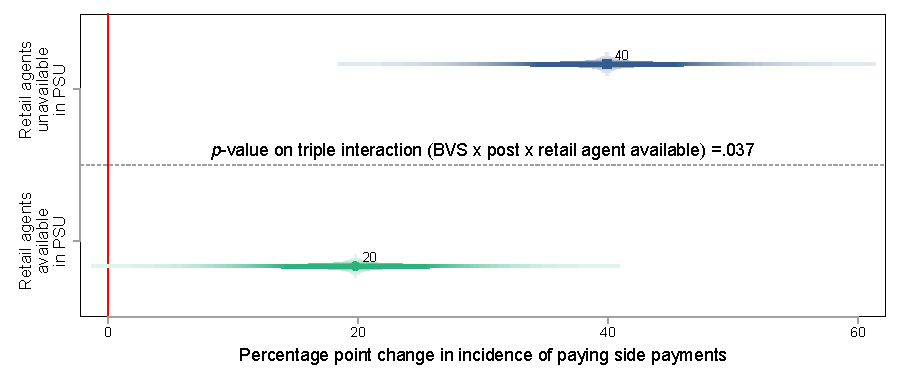
\includegraphics{coefplots/DD_HT_POS+bribes.pdf}} 
		\end{center}
		\hyperlink{pos_coverage}{\beamergotobutton{Map: baseline retail agent use}}
		\hyperlink{desc_graph}{\beamergotobutton{Corroboration from descriptive reports}} 
	\headlineextra{\footnotesize \textcolor{white}{Do not circulate}}
\end{frame}

%-------------------------------------------------------------------------


\begin{frame}{Woman has to visit payment point to scan fingerprint}
	Is female presence a possible mechanism for side payments result?
	\headlineextra{\footnotesize \textcolor{white}{Do not circulate}}
	\vspace{.2cm}
	\begin{itemize}
		\setlength\itemsep{.5em}
		\item \textbf{Reporting effect:} women now go in person so 
			  they have better knowledge of side payments
			  \pause
	    \item \textbf{Gender norms:} women now go in person and given strong 
		   	   gender norms, they are more susceptible to pressure from 
			   retail agents than their male representatives 
	\end{itemize}
	\vspace{.2cm}
	\pause
	Unlikely: we see the \textbf{same effect} on women who previously
		   \textbf{collected cash personally} in areas with baseline 
		   access to human retail agents
	\begin{center}
		{\scalebox{.75}{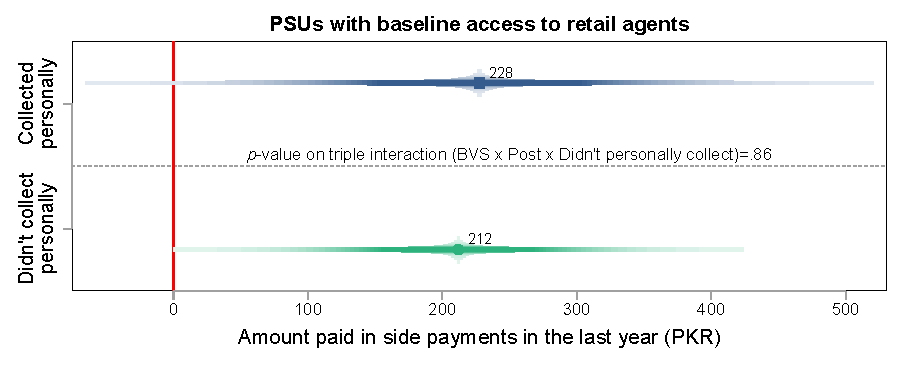
\includegraphics{DD_self_collected_total_bribes_pos}}} 
	\end{center}
\end{frame}



\begin{frame}{Increased coverage of retail agents reflected in reduced travel time}
	Areas with above median travel time at baseline see a large (but imprecise) 
	decrease in travel time post-treatment
	\vspace{-.4cm}
	\begin{table}
		\caption{\textbf{HTE by above median travel time at baseline}}
		\scalebox{.85}{\input{\tabdir HT_JQ08A_travel_time.tex}}
	\end{table}
	\headlineextra{\footnotesize \textcolor{white}{Do not circulate}}
\end{frame} 


%-------------------------------------------------------------------------


%-------------------------------------------------------------------------


%-------------------------------------------------------------------------

%-------------------------------------------------------------------------

\begin{frame}{Potential mechanisms for increased control: information asymmetry}
	\headlineextra{\footnotesize \textcolor{white}{Do not circulate}}
	\vspace{-.2cm}
		\vspace{.2cm}
		\begin{itemize}
%			\setlength\itemsep{1em}
			\item Cash amount is \textbf{increased periodically} for inflation, 
			and may \textbf{vary because of rounding}  
			\pause
			\item When men collect cash on behalf of female beneficiaries, 
			they may capture all or part of the amount without the woman's 
			knowledge. 
			\pause
			\item \textbf{Woman's presence} at payment point \textbf{reduces 
			this information asymmetry}
			\pause
			\item WIP: test whether effect varies when BVS transition happens 
			before vs. after an increase  
			\begin{table}
				\caption{\textbf{HTE by baseline collection of cash by female beneficiary}}
				\scalebox{.65}{\input{\tabdir 13_FE_HT_JQ04A_panel_control_over_cash.tex}}
			\end{table}
		\end{itemize}
\end{frame}

\begin{frame}{Potential mechanisms for increased control: behavioral labelling effect}	
	\headlineextra{\footnotesize \textcolor{white}{Do not circulate}}
		\begin{itemize}
			\setlength\itemsep{2em}
			\item When only women are allowed to collect the cash transfer, it may 
			signal to them and the household that the cash transfer is intended 
			for the woman
			\item Could be tested with lab-in-the-field style experiments 
		\end{itemize}
\end{frame}



%-------------------------------------------------------------------------

\begin{frame}{Potential mechanisms for dissatisfaction}
\headlineextra{\footnotesize \textcolor{white}{Do not circulate}}
\begin{itemize}
	\item Challenges for women traveling in public
	\vspace{.2cm}
	\begin{itemize}
		\setlength\itemsep{1em}
		\item BVS requires women to come in person but safety concerns and gender  
		norms may make it challenging for them to travel
		\pause
		\item However, there is no detectable difference in satisfaction between 
		women who collected personally at baseline versus women who did not 
	\end{itemize}
\end{itemize}
\begin{center}
	\scalebox{.8}{\hspace{-1.5cm}%
	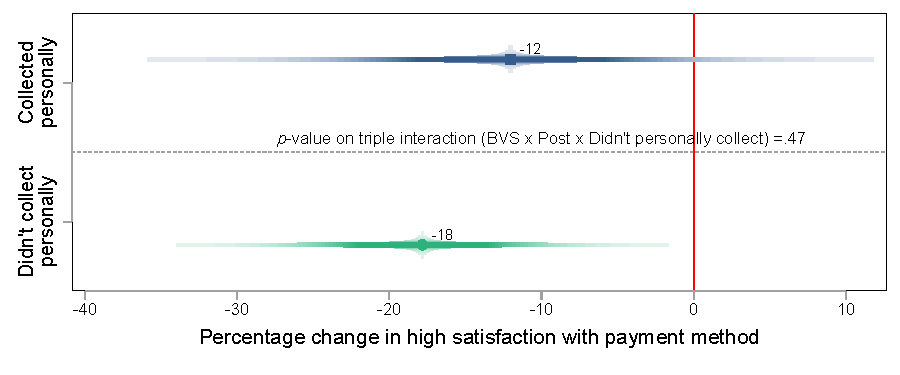
\includegraphics{coefplots/DD_self_collected_satisfaction}} 
\end{center}

\end{frame}

%-------------------------------------------------------------------------

\begin{frame}[label=sat_mech]{Potential mechanisms for dissatisfaction}
\headlineextra{\footnotesize \textcolor{white}{Do not circulate}}
\vspace{-.3cm}

\begin{itemize}
	\setlength\itemsep{1em}
	\item Increased \textbf{wait times} 
	\pause
	\begin{itemize}
		\setlength\itemsep{1em}
		\item Biometric authentication may take longer than debit card withdrawals
		\item Each beneficiary has to come in person whereas in control areas 
		one person can collect cash for multiple beneficiaries
		\item Strategic behavior by retail agents to solicit bribes  
	\end{itemize}
	\pause
	No baseline data on this, but at endline 10\% of beneficiaries 
	in BVS districts had to leave and return because of long wait times, vs 5\% in 
	non BVS \hyperlink{failures}{\beamergotobutton{Graph}}
	\pause
	\item \textbf{Biometric verification failures} 
	\begin{itemize}
		\setlength\itemsep{1em}
		\item Descriptively, in 2.3\% of cases, failure to collect cash within one 
		attempt is caused by biometric technology related issues 
		\hyperlink{failures}{\beamergotobutton{Graph}}
		\item However, BVS does not significantly increase the number of attempts 
		that have to be made to collect a given tranche \
		\hyperlink{attempts}{\beamergotobutton{Table}}
	\end{itemize}
	\pause
	\item \textbf{Additional time and money cost} for woman plus chaperone 
	traveling (Work in progress)
\end{itemize}
\end{frame}

%-------------------------------------------------------------------------
\begin{frame}{Increased coverage of human retail agents}
	\vspace{.2cm}
		\begin{itemize} 
		\item Increase in gross amount is not driven by increase in coverage 
		 	  of retail agents
		\item[] \textcolor{white}{Areas with less coverage at baseline see 
		a smaller increase in side payments}
		\item[] \textcolor{white}{Increased coverage of payment points may lower 
		side payments due to increased competition}
		\item[] \textcolor{white}{WIP: geocode new payment points to test this directly}
		\end{itemize} 
	\vspace{-.31cm}

	\begin{table}
		\caption{\textbf{HTE by above median travel time to payment point at baseline}}
		\scalebox{.7}{\input{\tabdir HT_JQ08A_panel_cash_received.tex}\hspace{2.8cm}}
	\end{table}
	
		\headlineextra{\footnotesize \textcolor{white}{Do not circulate}}
\end{frame} 

\setcounter{table}{3} \renewcommand{\thetable}{\arabic{table}}

\begin{frame}{Increased coverage of human retail agents}
	\vspace{.2cm}
		\begin{itemize} 
			\item Increase in gross amount is not driven by increase in coverage 
			 	  of retail agents
			\item Areas with less coverage at baseline see 
			a smaller increase in side payments
			\item Increased coverage of payment points may lower 
			side payments due to increased competition
			\item[] \textcolor{white}{WIP: geocode new payment points to test this directly}
		\end{itemize} 
	\vspace{-.31cm}
	\begin{table}
		\caption{\textbf{HTE by above median travel time to payment point at baseline}}
		\scalebox{.7}{\input{\tabdir HT_JQ08A_panel_cash_received_v2.tex}}
	\end{table}
	\headlineextra{\footnotesize \textcolor{white}{Do not circulate}}
\end{frame} 

\setcounter{table}{3} \renewcommand{\thetable}{\arabic{table}}

\begin{frame}{Increased coverage of human retail agents}
	\vspace{.2cm}
		\begin{itemize} 
			\item Increase in gross amount is not driven by increase in coverage 
			 	  of retail agents
			\item Areas with less coverage at baseline see 
			a smaller increase in side payments
			\item Increased coverage of payment points may lower 
			side payments due to increased competition
			\item WIP: geocode new payment points to test this directly
		\end{itemize} 
	\vspace{-.31cm}
	\begin{table}
		\caption{\textbf{HTE by above median travel time to payment point at baseline}}
		\scalebox{.7}{\input{\tabdir HT_JQ08A_panel_cash_received_v2.tex}}
	\end{table}
		\headlineextra{\footnotesize \textcolor{white}{Do not circulate}}
\end{frame} 


%%%%%%%%%%%%%%%%%%%%%%%%%%%%%%%%%%%%%%%%%%%%%%%%%%%%%%%%%%%%%%%%%%%%%%%%%%

\section{Conclusion and next steps}
\frame{\tableofcontents[currentsection]}

%-----------------------------------------------------------------------

\begin{frame}{Conclusion}
	\begin{itemize}
		\setlength\itemsep{2em}
		\item \textbf{Biometric technology} appears to \textbf{increase amount delivered} 
		\item Yet increase in \textbf{human involvement to operate the 
		technology cancelled these benefits}
		\item For \textbf{mobility constrained women}, biometric 
		verification systems \textbf{increased control over cash} 
		\item To \textbf{fully realize benefits of new technology}, need to address 
		\textbf{challenges raised} in its operation
	\end{itemize}
  	\headlineextra{\footnotesize \textcolor{white}{Do not circulate}}
  \end{frame}
  

%-----------------------------------------------------------------------
 
  \begin{frame}{Possible approaches to manage challenges}

	Ongoing analysis will inform policy recommendations - potential approaches 
	might include: 
  	
  	\begin{itemize}
  		\vspace{.2cm}
  		\setlength\itemsep{2em}
  		\item Further \textbf{expansion of payment point coverage} to reduce 
		travel time and increase competition between retail agents 
  		(BISP is working on this currently)
		\item \textbf{Biometric ATM expansion}
  		\item \textbf{Training / communication to beneficiaries} on account use, 
		and the amount of money they should expect to collect 
  		\item \textbf{Female retail agents} 
		\item \textbf{Mobile agents} 
  		\item Making \textbf{grievance redressal} processes more 
		accessible 
  	\end{itemize}
  	\headlineextra{\footnotesize \textcolor{white}{Do not circulate}}
  \end{frame}




%%%%%%%%%%%%%%%%%%%%%%%%%%%%%%%%%%%%%%%%%%%%%%%%%%%%%%%%%%%%%%%%%%%%%%%%%%

\section{Appendix}
\frame{\tableofcontents[currentsection]}

%-------------------------------------------------------------------------
\begin{frame}[label=balance]{Baseline balance (relative to districts with 0 BVS tranches)}
	\vspace{0cm}
	{\scalebox{.96}{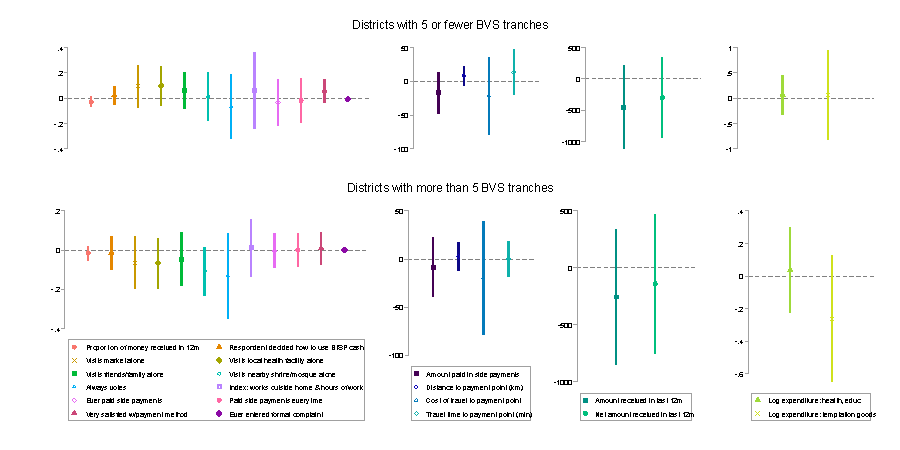
\includegraphics{coefplots/balance_coefplot}}}
	\hyperlink{methodology}{\beamergotobutton{Back to methodology}}
	\hyperlink{decay}{\beamergotobutton{Back to decay}}
	\headlineextra{\footnotesize \textcolor{white}{Do not circulate}}
\end{frame}


%\begin{frame}[label=balance]{Baseline balance ([1/2])}
%	\vspace{-.35cm}
%	\begin{table}
%		\caption{Balance table [1/2]}
%		\scalebox{.5}{\input{\tabdir 27_balance_BVS_startdate1.tex}}
%	\end{table}
%	\hyperlink{methodology}{\beamergotobutton{Back to methodology}}
%	\hyperlink{decay}{\beamergotobutton{Back to decay}}
%	\headlineextra{\footnotesize \textcolor{white}{Do not circulate}}
%\end{frame}
%
%\begin{frame}[label=balance]{Baseline balance [2/2]}
%	\vspace{-.35cm}
%	\begin{table}
%		\caption{Balance table [2/2]}
%		\scalebox{.48}{\input{\tabdir 27_balance_BVS_startdate2.tex}}
%	\end{table}
%	\hyperlink{methodology}{\beamergotobutton{Back to methodology}}
%	\hyperlink{decay}{\beamergotobutton{Back to decay}}
%	\headlineextra{\footnotesize \textcolor{white}{Do not circulate}}
%\end{frame}

%-------------------------------------------------------------------------
\begin{frame}[label=attrition]{Attrition}
\begin{table}
	\caption{\textbf{Test for differential attrition in OPM panel}}
	\scalebox{.9}{\input{\tabdir 21_attrition_v2.tex}}
\end{table}
	\hyperlink{survey}{\beamergotobutton{Back}}
\headlineextra{\footnotesize \textcolor{white}{Do not circulate}}
\end{frame}

%-------------------------------------------------------------------------
\begin{frame}[label=map]{Increase in side payments}
	\centering
			{\scalebox{.72}{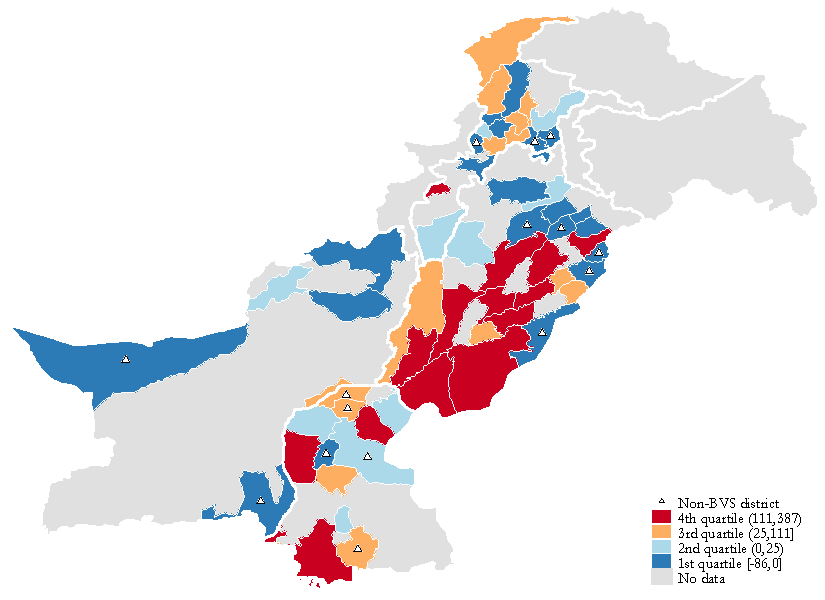
\includegraphics{panel_district_JQ11}}}
			\hyperlink{sidepayments}{\beamergotobutton{Back}}
	\headlineextra{\footnotesize \textcolor{white}{Do not circulate}}
\end{frame}

\begin{frame}[label=control]{Increase in percentage of women who personally  
	control BISP cash}
	\centering
			{\scalebox{.72}{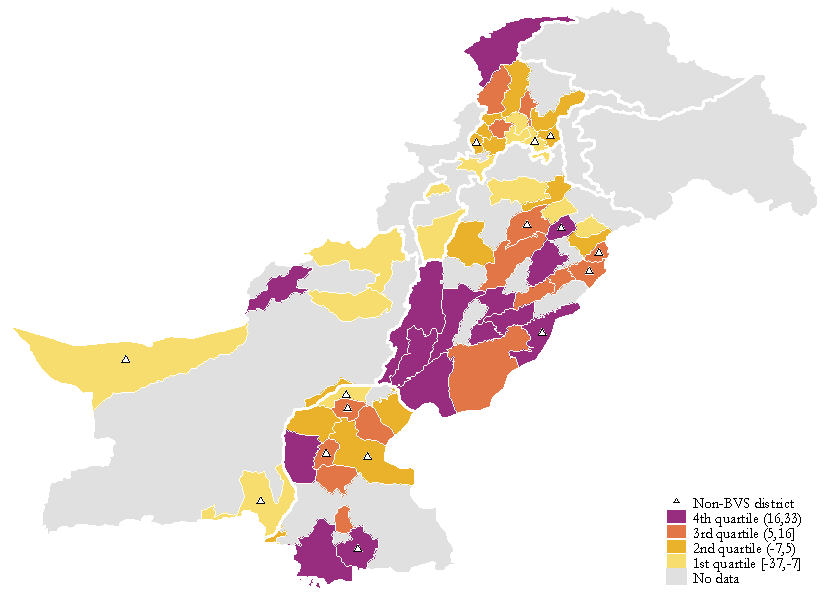
\includegraphics{panel_district_JQ18A_control}}}
			\hyperlink{control_map}{\beamergotobutton{Back}}
	\headlineextra{\footnotesize \textcolor{white}{Do not circulate}}
\end{frame}

%-------------------------------------------------------------------------
\begin{frame}[label=pos_coverage]{Percentage of people who use human retail 
	agents at baseline}
	\centering
			{\scalebox{.72}{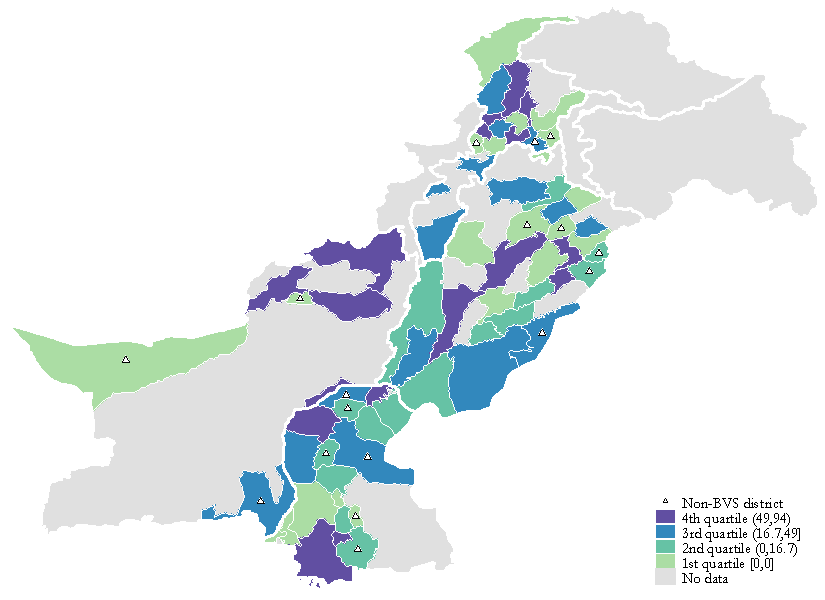
\includegraphics{panel_district_POS_use}}}
			\hyperlink{pos_hte}{\beamergotobutton{Back}}
	\headlineextra{\footnotesize \textcolor{white}{Do not circulate}}
\end{frame}


%-------------------------------------------------------------------------

\begin{frame}[label=failures]{Failures to withdraw cash are driven by biometric 
	technology failure in $\sim$2.3\% of cases}
	\vspace{-.5cm}
	\begin{center}
		\scalebox{.6}{\hspace{-1.5cm}%
			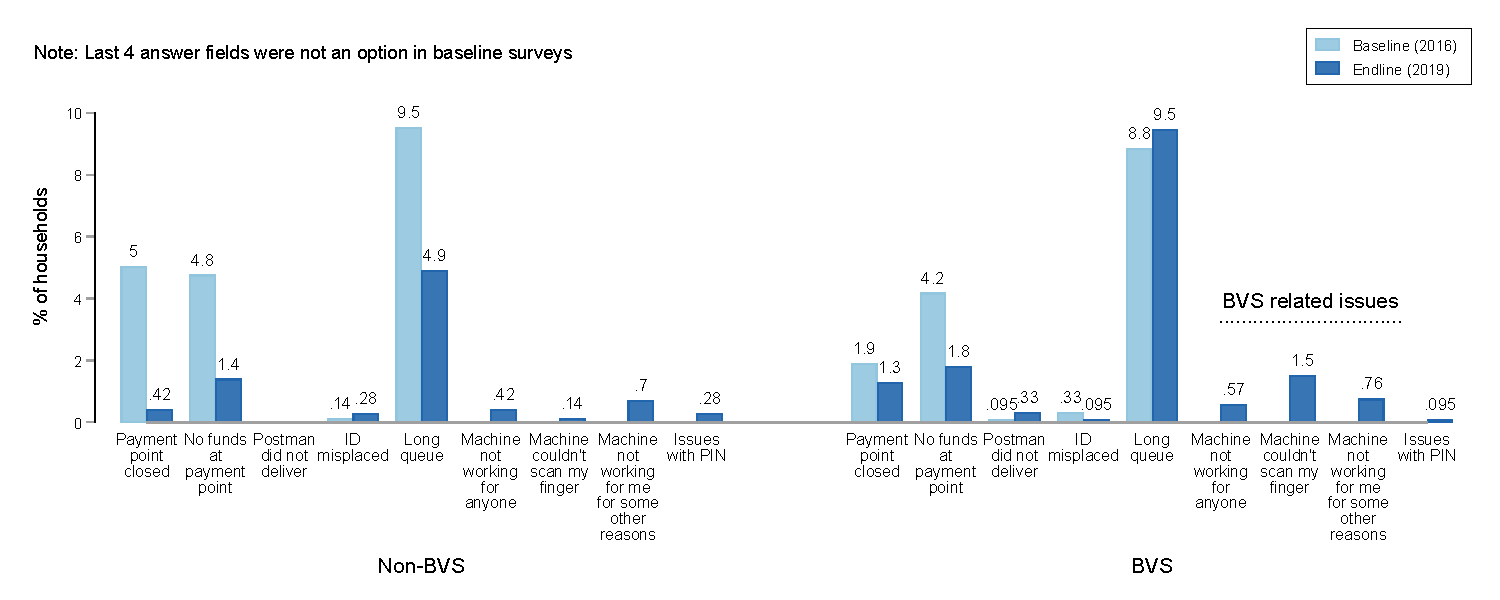
\includegraphics{panel_JQ14_failure_to_withdraw_to.pdf}}
	\end{center}
	\vspace{-.4cm}
		{\tiny This figure suggests that debit-card based districts have 
		seen an improvement in queueing time. We are investigating 
		whether this is due to infrastructural changes in debit-card 
		districts.\par}
		\hyperlink{sat_mech}{\beamergotobutton{Back}}
		\headlineextra{\footnotesize \textcolor{white}{Do not circulate}}
\end{frame}

%-------------------------------------------------------------------------

%-------------------------------------------------------------------------
\begin{frame}[label=bargraph]{Overall, no detectable change in net amount, after accounting 
	for increased side payments} 
			\begin{center}
				\vspace{-.1cm}
				\small Gross amount -- \textcolor{maroon}{travel cost}
				 -- \textcolor{maroon}{side payment} = Net amount
				\vspace{-.1cm}
				\scalebox{.62}{%
				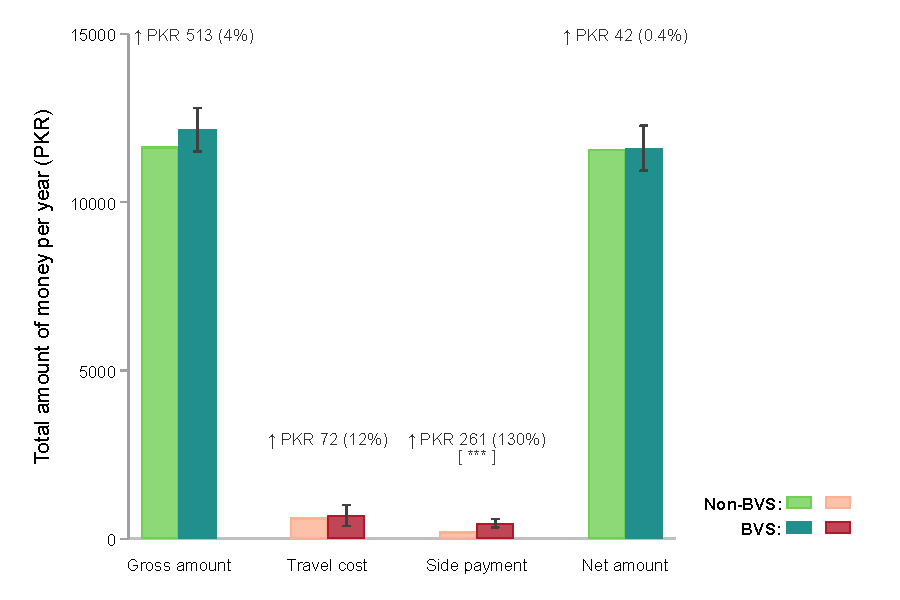
\includegraphics{net_of_costs_panel.pdf}}	
			\end{center}
				\vspace{-.4cm}
				
				{\scalebox{.6}{For reference, BISP households on average 
				have a per-adult equivalent monthly consumption 
				expenditure of PKR 3,064 or $\sim$USD 18.5 (\emph{Source: 
				OPM 2016 report}).  
				}\par}\vspace{-.1cm}
				
				{\scalebox{.6}{Note: The graphs show regression 
				coefficients, controlling for household and province-year 
				fixed effects. Standard errors clustered at 
				the district level.}\par}\vspace{-.1cm}
				
				{\scalebox{.6}{The asterisks [ * ] denote statistical 
				significance (* \emph{p} $<$.1, ** \emph{p} $<$.05, 
				*** \emph{p} $<$.01). Absence of asterisks 
				implies that we found no statistically detectable effect. 
				}\par}
	\hyperlink{sidepayments}{\beamergotobutton{Back}}					
	\headlineextra{\footnotesize \textcolor{white}{Do not circulate}}
\end{frame}

%-------------------------------------------------------------------------

\begin{frame}[label=net]{Effects similar (but noisier) for net amount}
	\vspace{.2cm}
		\begin{table}
			\caption{\textbf{HTE by baseline access to human retail agents}}
			\scalebox{.7}{\input{\tabdir HT_POS_avail_net_amount.tex}}
		\end{table}
		\hyperlink{gross}{\beamergotobutton{Back}}
	\headlineextra{\footnotesize \textcolor{white}{Do not circulate}}
\end{frame}

%-------------------------------------------------------------------------
\begin{frame}[label=attempts]{BVS does not increase number of attempts to collect cash transfer}
\begin{table}
	\caption{\textbf{Impact of BVS on number of attempts to collect cash transfer}}
	\scalebox{.75}{\input{\tabdir 10_FE_panel_cash_received.tex}}
\end{table}
\hyperlink{sat_mech}{\beamergotobutton{Back}}
\end{frame}

\end{document}